% Options for packages loaded elsewhere
\PassOptionsToPackage{unicode}{hyperref}
\PassOptionsToPackage{hyphens}{url}
\PassOptionsToPackage{dvipsnames,svgnames,x11names}{xcolor}
%
\documentclass[
  letterpaper,
  DIV=11,
  numbers=noendperiod]{scrartcl}

\usepackage{amsmath,amssymb}
\usepackage{lmodern}
\usepackage{iftex}
\ifPDFTeX
  \usepackage[T1]{fontenc}
  \usepackage[utf8]{inputenc}
  \usepackage{textcomp} % provide euro and other symbols
\else % if luatex or xetex
  \usepackage{unicode-math}
  \defaultfontfeatures{Scale=MatchLowercase}
  \defaultfontfeatures[\rmfamily]{Ligatures=TeX,Scale=1}
  \setmainfont[]{Times New Roman}
  \setsansfont[]{Times New Roman}
\fi
% Use upquote if available, for straight quotes in verbatim environments
\IfFileExists{upquote.sty}{\usepackage{upquote}}{}
\IfFileExists{microtype.sty}{% use microtype if available
  \usepackage[]{microtype}
  \UseMicrotypeSet[protrusion]{basicmath} % disable protrusion for tt fonts
}{}
\usepackage{xcolor}
\setlength{\emergencystretch}{3em} % prevent overfull lines
\setcounter{secnumdepth}{5}
% Make \paragraph and \subparagraph free-standing
\ifx\paragraph\undefined\else
  \let\oldparagraph\paragraph
  \renewcommand{\paragraph}[1]{\oldparagraph{#1}\mbox{}}
\fi
\ifx\subparagraph\undefined\else
  \let\oldsubparagraph\subparagraph
  \renewcommand{\subparagraph}[1]{\oldsubparagraph{#1}\mbox{}}
\fi


\providecommand{\tightlist}{%
  \setlength{\itemsep}{0pt}\setlength{\parskip}{0pt}}\usepackage{longtable,booktabs,array}
\usepackage{calc} % for calculating minipage widths
% Correct order of tables after \paragraph or \subparagraph
\usepackage{etoolbox}
\makeatletter
\patchcmd\longtable{\par}{\if@noskipsec\mbox{}\fi\par}{}{}
\makeatother
% Allow footnotes in longtable head/foot
\IfFileExists{footnotehyper.sty}{\usepackage{footnotehyper}}{\usepackage{footnote}}
\makesavenoteenv{longtable}
\usepackage{graphicx}
\makeatletter
\def\maxwidth{\ifdim\Gin@nat@width>\linewidth\linewidth\else\Gin@nat@width\fi}
\def\maxheight{\ifdim\Gin@nat@height>\textheight\textheight\else\Gin@nat@height\fi}
\makeatother
% Scale images if necessary, so that they will not overflow the page
% margins by default, and it is still possible to overwrite the defaults
% using explicit options in \includegraphics[width, height, ...]{}
\setkeys{Gin}{width=\maxwidth,height=\maxheight,keepaspectratio}
% Set default figure placement to htbp
\makeatletter
\def\fps@figure{htbp}
\makeatother
\newlength{\cslhangindent}
\setlength{\cslhangindent}{1.5em}
\newlength{\csllabelwidth}
\setlength{\csllabelwidth}{3em}
\newlength{\cslentryspacingunit} % times entry-spacing
\setlength{\cslentryspacingunit}{\parskip}
\newenvironment{CSLReferences}[2] % #1 hanging-ident, #2 entry spacing
 {% don't indent paragraphs
  \setlength{\parindent}{0pt}
  % turn on hanging indent if param 1 is 1
  \ifodd #1
  \let\oldpar\par
  \def\par{\hangindent=\cslhangindent\oldpar}
  \fi
  % set entry spacing
  \setlength{\parskip}{#2\cslentryspacingunit}
 }%
 {}
\usepackage{calc}
\newcommand{\CSLBlock}[1]{#1\hfill\break}
\newcommand{\CSLLeftMargin}[1]{\parbox[t]{\csllabelwidth}{#1}}
\newcommand{\CSLRightInline}[1]{\parbox[t]{\linewidth - \csllabelwidth}{#1}\break}
\newcommand{\CSLIndent}[1]{\hspace{\cslhangindent}#1}

%\documentclass{article}

% todonotes package                          #####################

\usepackage[textsize=footnotesize]{todonotes}


%language                                    #####################

%\usepackage{times}
%\usepackage{t1enc}                               Trouble maker
%\usepackage[utf8x]{inputenc}
%\usepackage[polish]{babel}
%\usepackage{polski}


% math                                       #####################

%AMS
\usepackage{amsfonts}
\usepackage{amssymb}
\usepackage{amsthm}
\usepackage{amsmath}
\usepackage{mathtools}


% quote environment                        #######################  Unfortunately it destroys the font, only an issue in a mathmode

%\usepackage[T1]{fontenc} % Required for correct quotes with ""

%\renewenvironment{quote}
%{\list{}{\leftmargin=1em\rightmargin=1em}\item[]``}
%{''\endlist}



% page geometry                              #####################


\usepackage{geometry}
 \geometry{a4paper,left=35mm,top=20mm,}

\setlength{\parindent}{10pt}
\setlength{\parskip}{1pt}

\usepackage{float}
\restylefloat{figure}

% abbreviations                              #####################

\newcommand{\ra}{\rangle}
\newcommand{\la}{\langle}
\newcommand{\n}{\neg}
\newcommand{\et}{\wedge}
\newcommand{\jt}{\rightarrow}
\newcommand{\ko}[1]{\forall  #1\,}
\newcommand{\ro}{\leftrightarrow}
\newcommand{\exi}[1]{\exists\, {_{#1}}}
\newcommand{\pr}[1]{\mathsf{P}(#1)}
\newcommand{\cost}{\mathsf{cost}}
\newcommand{\benefit}{\mathsf{benefit}}
\newcommand{\ut}{\mathsf{ut}}

\newcommand{\dkl}{D_{\mathsf{KL}}} % trying to add the definition of \dkl

\newcommand{\odds}{\mathsf{Odds}}
\newcommand{\ind}{\mathsf{Ind}}
\newcommand{\nf}[2]{\nicefrac{#1\,}{#2}}
\newcommand{\R}[1]{\texttt{#1}}
\newcommand{\prr}[1]{\mbox{$\mathtt{P}_{prior}(#1)$}}
\newcommand{\prp}[1]{\mbox{$\mathtt{P}_{posterior}(#1)$}}

\newcommand{\s}[1]{\mbox{$\mathsf{#1}$}}


\newtheorem{q}{\color{blue}Question}
\newtheorem{lemma}{Lemma}


\newtheorem{theorem}{Theorem}
\newtheorem{definition}{Definition}        % trying to add the def. environment



% bibliography                                #####################

%\usepackage[authoryear]{natbib}  % solution to the  natbib compilation error

%\bibliographystyle{apalike}





\KOMAoption{captions}{tableheading}
\makeatletter
\makeatother
\makeatletter
\makeatother
\makeatletter
\@ifpackageloaded{caption}{}{\usepackage{caption}}
\AtBeginDocument{%
\ifdefined\contentsname
  \renewcommand*\contentsname{Table of contents}
\else
  \newcommand\contentsname{Table of contents}
\fi
\ifdefined\listfigurename
  \renewcommand*\listfigurename{List of Figures}
\else
  \newcommand\listfigurename{List of Figures}
\fi
\ifdefined\listtablename
  \renewcommand*\listtablename{List of Tables}
\else
  \newcommand\listtablename{List of Tables}
\fi
\ifdefined\figurename
  \renewcommand*\figurename{Figure}
\else
  \newcommand\figurename{Figure}
\fi
\ifdefined\tablename
  \renewcommand*\tablename{Table}
\else
  \newcommand\tablename{Table}
\fi
}
\@ifpackageloaded{float}{}{\usepackage{float}}
\floatstyle{ruled}
\@ifundefined{c@chapter}{\newfloat{codelisting}{h}{lop}}{\newfloat{codelisting}{h}{lop}[chapter]}
\floatname{codelisting}{Listing}
\newcommand*\listoflistings{\listof{codelisting}{List of Listings}}
\makeatother
\makeatletter
\@ifpackageloaded{caption}{}{\usepackage{caption}}
\@ifpackageloaded{subcaption}{}{\usepackage{subcaption}}
\makeatother
\makeatletter
\@ifpackageloaded{tcolorbox}{}{\usepackage[many]{tcolorbox}}
\makeatother
\makeatletter
\@ifundefined{shadecolor}{\definecolor{shadecolor}{rgb}{.97, .97, .97}}
\makeatother
\makeatletter
\makeatother
\ifLuaTeX
  \usepackage{selnolig}  % disable illegal ligatures
\fi
\IfFileExists{bookmark.sty}{\usepackage{bookmark}}{\usepackage{hyperref}}
\IfFileExists{xurl.sty}{\usepackage{xurl}}{} % add URL line breaks if available
\urlstyle{same} % disable monospaced font for URLs
\hypersetup{
  pdftitle={Second-order Probabilism: Expressive Power and Accuracy},
  pdfauthor={Rafal Urbaniak and Marcello Di Bello},
  colorlinks=true,
  linkcolor={blue},
  filecolor={Maroon},
  citecolor={Blue},
  urlcolor={Blue},
  pdfcreator={LaTeX via pandoc}}

\title{Second-order Probabilism: Expressive Power and Accuracy}
\author{Rafal Urbaniak and Marcello Di Bello}
\date{2024-02-28}

\begin{document}
\maketitle
\ifdefined\Shaded\renewenvironment{Shaded}{\begin{tcolorbox}[sharp corners, borderline west={3pt}{0pt}{shadecolor}, frame hidden, boxrule=0pt, interior hidden, enhanced, breakable]}{\end{tcolorbox}}\fi

\renewcommand*\contentsname{Table of contents}
{
\hypersetup{linkcolor=}
\setcounter{tocdepth}{3}
\tableofcontents
}
\vspace{2cm}

\noindent \textbf{DISCLAIMER:}
\textbf{This is a draft of work in progress, please do not cite or distribute without permission.}

\thispagestyle{empty}

\newpage

\begin{quote} \textbf{Abstract.}  \todo{need to write one when done}

\end{quote}

\hypertarget{introduction}{%
\section{Introduction}\label{introduction}}

\label{sec:introduction}

As rational agents, we form beliefs about a variety of propositions on
the basis of the evidence available to us. But believing a proposition
is not an all-or-nothing affair; it is a matter of degrees. We are
uncertain, to a greater or lesser extent, about the truth of many
propositions since the evidence we possess about them is often fallible.
To represent this uncertainty, it is natural to use a probability
measure that assigns to each proposition a value between 0 and 1 (also
called a degree of belief or credence). This approach---known as
\emph{precise probabilism}---models an agent's state of uncertainty (or
credal state) with a single probability measure: each proposition is
assigned one probability value (a sharp degree of belief). The problem
is that a sharp probability measure is not expressive enough to
distinguish between intuitively different states of uncertainty rational
agents may find themselves in (\S \ref{sec:precise-probabilism}). To
avoid this problem, a \emph{set} of probability measures, rather than a
single one, can be used to represent the uncertainty of a rational
agent. This approach is known as \emph{imprecise probabilism}. It
outperforms precise probabilism in some respects, but also runs into
problems of its own (\S \ref{sec:imprecise-probabilism}).

To make progress, this paper argues that the uncertainty of a rational
agent is to be represented neither by a single probability measure nor a
set of measures. Rather, it is to be represented by a higher-order
probability measure, more specifically, a probability distribution over
parameter values intepreted as probabilities. Call this view
\emph{higher-order probabilism}. We show that higher-order probabilism
addresses all the problems and philosophical puzzles that plague both
precise and imprecise probabilism (\S \ref{sec:higher-order} and
\S \ref{sec:proper-scores}).

Moreover, Bayesian probabilistic programming already provides a fairly
reliable implementation framework of this approach.

\todo{add structure description}

\todo{Think about including synergy}

\hypertarget{precise-probabilism}{%
\section{Precise probabilism}\label{precise-probabilism}}

\label{sec:precise-probabilism}

Precise probabilism (\textsf{PP}) holds that a rational agent's
uncertainty about a proposition is to be represented as a single,
precise probability measure. Bayesian updating regulates how the prior
probability measure should change in light of new evidence that the
agent learns. The updating can be iterated multiple times for multiple
pieces of evidence considered successively. This is an elegant and
simple theory with many powerful applications. Unfortunately,
representing our uncertainty about a proposition in terms of a single,
precise probability measure runs into a number of difficulties.

Precise probabilism fails to capture an important dimension of how our
fallible beliefs reflect the evidence we have (or have not) obtained. A
couple of stylized examples featuring coin tosses should make the point
clear.

\begin{quote}
\textbf{No evidence v. fair coin}
You are about to toss a coin, but have no evidence 
about its bias. You are completely ignorant. 
Compare this to the situation in which you know, 
based on overwhelming evidence, that the coin is fair. 
\end{quote}

\noindent On precise probabilism, both scenarios are represented by
assigning a probability of .5 to the outcome \emph{heads}. If you are
completely ignorant, the principle of insufficient evidence suggests
that you assign .5 to both outcomes. Similarly, if you know for sure the
coin is fair, assigning .5 seems the best way to quantify the
uncertainty about the outcome. The agent's evidence in the two scenarios
is quite different, but precise probabilities fail to capture this
difference.

\begin{quote}
\textbf{Learning from ignorance}
You toss a coin with unknown bias. You toss it 10 times and observe \emph{heads} 5 times. Suppose you toss it further and observe 50 \emph{heads} in 100 tosses. 
\end{quote}

\noindent Since the coin initially had unknown bias, you should
presumably assign a probability of .5 to both outcomes if you stick with
precise probabilism. After the 10 tosses, you again assess the
probability to be .5. You must have learned something, but whatever that
is, it is not modeled by precise probabilities. When you toss the coin
100 times and observe 50 heads, you learn something new as well. But
your precise probability assessment will again be .5.

These examples suggest that precise probabilism is not appropriately
responsive to evidence. Representing an agent's uncertainty by a precise
probability measure can fail to track what an agent has learned from new
evidence. Precise probabilism assigns the same probability in situations
in which one's evidence is quite different: when no evidence is
available about a coin's bias; when there is little evidence that the
coin is fair (say, after only 10 tosses); and when there is strong
evidence that the coin is fair (say, after 100 tosses). In fact,
analogous problems also arise for evidence that the coin is not fair.
Suppose the rational agent starts with a weak belief that the coin is .6
biased towards heads. They can strengthen that belief by tossing the
coin repeatedly and observing, say, 60 heads in 100 tosses. But this
improvement in their evidence is not mirrored in the .6 probability they
are supposed to assign to \emph{heads}.\footnote{Here is another problem
  for precise probabilism. Imagine a rational agent who does not know
  the bias of the coin. For precise probabilism, this state of
  uncertainty should be represented by a .5 probability assignment to
  the \emph{heads}. Next, the agent learns that the bias towards heads,
  whatever the bias is, has been slightly increased, say by .001. The
  addition of this new information is called \emph{sweetening} in the
  philosophical literature. This sweetening should now make the agent
  bet on heads: if the probability of \emph{heads} was initially .5, it
  must be ever so slightly above .5 after sweetening. But, intuitively,
  the new information should leave the agent equally undecided about
  betting on heads or tails. After sweetening, the agent still does not
  know much about the actual bias of the coin.}
\todo{add reference about sweetening}

These problems generalize beyond cases of coin tossing. It is one thing
not to know much about whether a proposition is true, for example,
whether an individual is guilty of a crime. It is another thing to have
strong evidence that favors a hypothesis and equally strong evidence
that favors its negation, for example, strong evidence favoring the
guilt hypothesis and equally strong evidence favoring the hypothesis of
innocence. Despite this difference, precise probabilism would reccomend
that a probability of .5 be assigned to both hypotheses in either case.
Here, too, precise probabilities fail to be appropriately responsive to
the evidence.

In addition, evidence can accumulate in a way that does not require
changing our initial probability assignments. Suppose that, at first,
one's overall evidence favors \(A\) over \(B\). So the probability
assigned to \(A\) should be greater than that assigned to \(B\). Next,
the agent acquires new evidence. The total quantity of evidence has
increased, but suppose this larger body of evidence overall still favors
\(A\) over \(B\). So no change in the probabilities seems required.
Still, something has changed about the agent's state of uncertainty
towards \(A\) and \(B\): the quantity of evidence on which the agent can
make their assessment whether \(A\) is more probable than \(B\) has
become larger. And yet, this change in the quantity of overall evidence
is not reflected in the precise probabilities assigned to the
propositions \(A\) and \(B\).\footnote{Following Keynes, the distinction
  here is between the \emph{balance} of the evidence---whether the
  evidence available tips in favor a proposition or another---and the
  \emph{weight} of the evidence---the overall quantity of evidence.
  \textbf{ADD REFRENCE TO KEYNES}}

\hypertarget{imprecise-probabilism}{%
\section{Imprecise probabilism}\label{imprecise-probabilism}}

\label{sec:imprecise-probabilism}

What if we give up the assumption that probability assignments should be
precise? Imprecise probabilism (\textsf{IP}) holds that a rational
agent's credal stance towards a hypothesis is to be represented by a
\emph{set of probability measures}, typically called a representor
\(\mathbb{P}\), rather than a single measure \(\mathsf{P}\). The
representor should include all and only those probability measures which
are compatible with the evidence (more on this point later).\footnote{For
  the development of imprecise probabilism, see Keynes (1921); Levi
  (1974); Gärdenfors \& Sahlin (1982); Kaplan (1968); Joyce (2005);
  Fraassen (2006); Sturgeon (2008); Walley (1991). Bradley (2019) is a
  good source of further references. Imprecise probabilism shares some
  similarities with what we might call \textbf{interval probabilism}
  (Kyburg, 1961; Kyburg Jr \& Teng, 2001). On interval probabilism,
  precise probabilities are replaced by intervals of probabilities. On
  imprecise probabilism, instead, precise probabilities are replaced by
  sets of probabilities. This makes imprecise probabilism more general,
  since the probabilities of a proposition in the representor set do not
  have to form a closed interval.} It is easy to see that modeling an
agent's credal state by sets of probability measures avoids some of the
shortcomings of precise probabilism. For instance, if an agent knows
that the coin is fair, their credal state would be represented by the
singleton set \(\{\mathsf{P}\}\), where \(\mathsf{P}\) is a probability
measure that assigns \(.5\) to \emph{heads}. If, on the other hand, the
agent knows nothing about the coin's bias, their credal state would be
represented by the set of all probabilistic measures, since none of them
is excluded by the available evidence. Note that the set of probability
measures does not represent admissible options that the agent could
legitimately pick from. Rather, the agent's credal state is essentially
imprecise and should be represented by means of the entire set of
probability measures.

So far so good. But, just as precise probabilism fails to be
appropriately evidence-responsive in certain scenarios, imprecise
probabilism runs in similar difficulties in other scenarios.

\begin{quote}
\textbf{Even v. uneven bias:}
 You have two coins and you know, for sure, that the probability of getting heads is .4, if you toss one coin, and .6, if you toss the other coin. But you do not know which is which. You pick one of the two at random and toss it.  Contrast this with an uneven case. You have four coins and you know that three of them have bias $.4$ and one of them has bias $.6$. You pick a coin at random and plan to toss it. You should be three times more confident that the probability of getting heads is .4. rather than .6.
\end{quote}

\noindent The first situation can be easily represented by imprecise
probabilism. The representor would contain two probability measures, one
that assigns .4. and the other that assigns .6 to the hypothesis `this
coin lands heads'. But imprecise probabilism cannot represent the second
situation. Since the probability measures in the set are all compatible
with the agent's evidence, no probability measure can be assigned a
greater (higher-order) probability than any other.\footnote{Other
  scenarios can be constructed in which imprecise probabilism fails to
  capture distinctive intuitions about evidence and uncertainty; see,
  for example, (Rinard, 2013). Suppose you know of two urns,
  \textsf{GREEN} and \textsf{MYSTERY}. You are certain \textsf{GREEN}
  contains only green marbles, but have no information about
  \textsf{MYSTERY}. A marble will be drawn at random from each. You
  should be certain that the marble drawn from \textsf{GREEN} will be
  green (\(G\)), and you should be more confident about this than about
  the proposition that the marble from \textsf{MYSTERY} will be green
  (\(M\)). In line with how lack of information is to be represented on
  \textsf{IP}, for each \(r\in [0,1]\) your representor contains a
  \(\mathsf{P}\) with \(\pr{M}=r\). But then, it also contains one with
  \(\pr{M}=1\). This means that it is not the case that for any
  probability measure \(\mathsf{P}\) in your representor,
  \(\mathsf{P}(G) > \mathsf{P}(M)\), that is, it is not the case that RA
  is more confident of \(G\) than of \(M\). This is highly
  counter-intuitive.}

These examples show that imprecise probabilism is not expressive enough
to model the scenario of uneven bias. Defenders of imprecise probabilism
could concede this point but prefer their account for reasons of
simplicity. They could also point out that imprecise probabilism models
scenarios that precise probabilism cannot model, for example, a state of
complete lack of evidence. In this respect, imprecise probabilism
outperforms precise probabilism in expressive power, but also retains
theoretical simplicity. Unfortunately, it is questionable whether
imprecise probabilism outperforms precise probabilism \emph{all things
considered}. In fact, imprecise probabilism suffers from a number of
shortcomings that do not affect precise probabilism.

The first shortcoming has not received extensive discussion in the
literature, but it is fundamental. Recall that, for imprecise
probabilism, an agent's state of uncertainty is represented by those
probability measures that are \emph{compatible} with the agent's
evidence. The question is, how should the notion of compatibility be
understood here? Perhaps we can think of compatibility as the fact that
the agent's evidence is consistent with the probability measure in
question. But mere consistency wouldn't get the agent very far in
excluding probability measures, as too many probability measures are
strictly speaking still consistent with most observations and data.
Admittedly, there will be clear-cut cases: if you see the outcome of a
coin toss to be heads, you reject the measure with \(\mathsf{P}(H)=0\),
and similarly for tails. Another class of cases might arise while
randomly drawing objects from a finite set where the true frequencies or
objective chances are already known, because the finite set has been
inspected. But such clear-cut cases aside, what else? In the end,
evidence will often be consistent with almost any probability
measure.\footnote{Probability measures can be inconsistent with
  evidential constraints that agents believe to be true. Mathematically,
  non-trivial evidential constraints are easy to model (Bradley, 2012).
  They can take the form, for example, of the \emph{evidence of chances}
  \(\{ \mathsf{P}(X) = x\}\) or \(\mathsf{P}(X) \in [x,y]\), or
  \emph{structural constraints} such as ``\(X\) and \(Y\) are
  independent'' or ``\(X\) is more likely than \(Y\).'' These
  constraints are something that an agent can come to accept outright,
  but only if offered such information by an expert whom the agent
  completely defers to. But, besides these idealized cases, it is
  unclear how an agent could come to accept such structural constraints
  upon observation. There will usually be some degree of uncertainty
  about the acceptability of these constraints.}

A second, well-known problem for imprecise probabilism is belief
inertia. Precise probabilism offers an elegant model of learning from
evidence: Bayesian updating. Imprecise probabilism, at least
\emph{prima facie}, offers an equally elegant model of learning from
evidence, richer and more nuanced. It is a natural extension of the
classical Bayesian approach that uses precise probabilities. When faced
with new evidence \(E\) between time \(t_0\) and \(t_1\), the
representor set should be updated point-wise, running the standard
Bayesian updating on each probability measure in the representor:
\begin{align*} \label{eq:updateRepresentor}
\mathbb{P}_{t_1} = \{\mathsf{P}_{t_1}\vert \exists\, {\mathsf{P}_{t_0} \!\in  \mathbb{P}_{t_0}}\,\, \forall\, {H}\,\, \left[\mathsf{P}_{t_1}(H)=\mathsf{P}_{t_0}(H \vert E)\right] \}.
\end{align*}

\noindent The hope is that, if we start with a range of probabilities
that is not extremely wide, point-wise learning will behave
appropriately. For instance, if we start with a prior probability of
\emph{heads} equal to .4 or .6, then those measures should be updated to
something closer to \(.5\) once we learn that a given coin has already
been tossed ten times with the observed number of heads equal 5 (call
this evidence \(E\)). This would mean that if the initial range of
values was \([.4,.6]\) the posterior range of values should be narrower.

Unfortunately, this narrowing of the range of values becomes impossible
whenever the starting point is complete lack of knowledge, as imprecise
probabilism runs into the problem of belief inertia (Levi, 1980). This
problem arises in situations in which no amount of evidence could lead
the agent to change their belief state, according to a given modeling
strategy. Consider a situation in which you start tossing a coin knowing
nothing about its bias. The range of possibilities is \([0,1]\). After a
few tosses, if you observed at least one tail and one heads, you can
exclude the measures assigning 0 or 1 to \emph{heads}. But what else
have you learned? If you are to update your representor set point-wise,
you will end up with the same representor set. For any sequence of
outcomes that you can obtain and any probability value in \([0, 1],\)
there will exist a probability measure (conditional on the oucomes) that
assigns that probability to \emph{heads}. Consequently, the edges of
your resulting interval will remain the same. In the end, it is not
clear how you are supposed to learn anything if you start from complete
ignorance.\footnote{Here's another example of inertia, coming from
  Rinard (2013). Either all the marbles in the urn are green (\(H_1\)),
  or exactly one tenth of the marbles are green (\(H_2\)). Suppose your
  initial credence about these two hypothesis is complete uncertainty
  with interval. Next, suppose you learn that a marble drawn at random
  from the urn is green (\(E\)). After using this evidence to condition
  each probability measure in your representor (which initially contains
  all possible probability measures over the relevant space) on this
  evidence, you end up with the same spread of values for \(H_1\) that
  you had before learning \(E\). This holds no matter how many marbles
  are sampled from the urn and found to be green. This is
  counterintuitive: if you continue drawing green marbles, even if you
  started with complete uncertainty, you should become more inclided
  towards the hypothesis that all marbles are green.}

Some downplay the problem of belief inertia. After all, if you started
with knowing truly nothing, then it is right to conclude that you will
never learn anything. Joyce (2010) writes:

\begin{quote}
You cannot learn anything in cases of pronounced ignorance simply
because a prerequisite for learning is to have prior views about how
potential data should alter your beliefs (p.~291)
\todo{add reference.Joyce, J. M. (2010). A Defence of Imprecise Credences in Inference and Decision
Making, *Philosophical Perspectives* 24, pp. 281–323.}
\end{quote}

\noindent The upshot is that vacuous priors should not be used and that
imprecise probabilism gives the right results when the priors are
non-vacuous.

\todo{Actually moved Moss here and replied to joyce as well, review and discuss.}

This is in line with Moss CITE, who suggests a potential way out for the
impreciser. Just like regularity constraint (do not accept prior that
sets probabilities 1 or 0 to contingent claims) may be reasonable, so
may be a more general constraint to not accept priors about contingent
proporitions that are unrevisable also in the imprecise case. The recipe
seems simple enough. Do you get stuck when starting with too wide
priors? Don't start there! The challenge, however, is to explain in
principled manner what other priors in the inertia examples the agent is
justified in taking and why. Morevoer, avoiding belief inertia by
walking around it will not help us with other difficulties with
imprecise probabilism. Moreover, while it is true that you cannot learn
anything in the state of pronounced ignorance, the usual examples of
inertia are not of that sort. Yes, we are completely ignorant of what,
say, the coin bias is, but we also know enough to reason about how our
convictions would change in light of evidence. We know the coin is
two-sided, we know the bias doesn't change between the tosses, etc.. In
general, we are justified in using the assumptions that we actually do
use to show how a higher order probabilist can learn the bias from
observations even if they start from a uniform prior about that
parameter.

\todo{Rafal to develop a response to this point.} Another strategy is to
say that, in a state of complete ignorance, a special updating rule
should be deployed.\footnote{Elkin (2017) suggests the rule of
  \emph{credal set replacement} that recommends that upon receiving
  evidence the agent should drop measures rendered implausible, and add
  all non-extreme plausible probability measures. This, however, is
  tricky. One needs a separate account of what makes a distribution
  plausible from a principled account of why one should use a separate
  special update rule when starting with complete ignorance.}

Finally, imprecise probabilism faces a third, deeper problem that does
not arise for precise probabilism. As it turns out, it is impossible to
define proper scoring rules for measuring the accuracy of a representor.
Workable \emph{scoring rules} exist for measuring the accuracy of a
single, precise probability measure, such as the Brier score. These
rules measure the distance between a rational agent's probability
measure and the actual value. A requirement of scoring rules is that
they be \emph{proper}: any rational agent will expect their own
probability measure to be more accurate than any other. After all, if an
agent thought a different probability measure was more accurate, they
should switch to it. Proper scoring rules are then used to formulate
accuracy-based arguments for precise probabilism. These arguments show
(roughly) that, if your precise measure follows the axioms of
probability theory, no other non-probabilistic measure is going to be
more accurate than yours whatever the facts are. Can the same be done
for imprecise probabilism? It cannot. Impossibility theorems demonstrate
that no proper scoring rules are available for representor sets
(Seidenfeld, Schervish, \& Kadane, 2012). So, as many have noted, the
prospects for an accuracy-based argument for imprecise probabilism look
dim (Campbell-Moore, 2020; Mayo-Wilson \& Wheeler, 2016). Moreover, as
shown by Schoenfield (2017), if an accuracy measure satisfies certain
plausible formal constraints, it will never strictly recommend an
imprecise stance, as for any imprecise stance there will be a precise
one with at least the same accuracy.

\hypertarget{higher-order-probabilism}{%
\section{Higher-order probabilism}\label{higher-order-probabilism}}

\label{sec:higher-order}

Let us take stock. Imprecise probabilism is more expressive than precise
probabilism. It can model the difference between a state in which there
is no evidence about a proposition (or its negation) and a state in
which the evidence for and against a proposition is in equipoise. But
imprecise probabilism has its own expressive limitations, for example,
it cannot model the case of uneven bias. In addition, imprecise
probabilism faces difficulties that do not affect precise probabilism:
the notion of compatibility between a probability measure and the
evidence is too permissive; belief inertia makes it impossible for a
rational agent to learn via Bayesian updating; and no proper scoring
rules exist for imprecise probabilism. In this section, we show that
higher-order probabilism overcomes the expressive limitations of
imprecise probabilism without falling prey to any such difficulties.

Proponents of imprecise probabilism already hinted at the need of
relying on higher order-probabilities. For instance, Bradley compares
the measures in a representor to committee members, each voting on a
particular issue, say the true chance or bias of a coin. As they acquire
more evidence, the committee members will often converge on a chance
hypothesis.

\begin{quote}
\dots the committee members are ``bunching up''. Whatever measure you
put over the set of probability functions---whatever ``second order
probability'' you use---the ``mass'' of this measure gets more and more
concentrated around the true chance hypothesis. (Bradley, 2012, p. 157)
\end{quote}

\noindent But such bunching up cannot be modeled by imprecise
probabilism alone: a probability distribution over chance hypotheses is
needed.\footnote{In a similar vein, Joyce (2005), in a paper defending
  imprecise probabilism, explicates the notion of weight of evidence
  using a probability distribution over chance hypotheses. Oddly,
  representor sets play no central role in Joyce's account of the weight
  of evidence.} That one should use higher-order probabilities has also
been suggested by critics of imprecise probabilism. For example, Carr
(2020) argues that sometimes evidence requires uncertainty about what
credences to have. Carr, however, does not articulate this suggestion
more fully; does not develop it formally; and does not explain how her
approach would fare against the difficulties affecting precise and
imprecise probabilism. We now set out to do precisely that.

\todo{Rafal to correct technical mistakes in this paragraph (e.g. concept of distribution over probability measures seems incorrect for our purposes)}
\todo{Revised this bit, take a look.}

The central idea of higher-order probabilism is this: a rational agent's
uncertainty is not single-dimensional and thus cannot be mapped onto a
one-dimensional scale such as the real line. Uncertainty is best modeled
by the shape of a probability distribution, sometimes even over the
parameters which are best construed as probabilities themselves. In some
straighforward cases of narrow and symmetric distributions we can get
away with using point estimates, but such approximations will fail to be
useful in more complex cases.

Stated more formally, a rational agent's state of uncertainty (or credal
stance) towards a proposition \(X\) is not represented by a single
probability value \(\mathsf{P}(X)\) between 0 and 1, but by a
probability density \(f(\mathsf{P}(X))\), where the first-order
probability of \(X\) is the parameter in question, and is treated as a
random variable. Crucially, this representation is quite general. While
the examples used so far may not indicate this, the proposition \(X\) is
not restricted to chance hypotheses or the bias of a coin. The
probability density \(f(\mathsf{P}(X))\) assigns a second-order
probability (density) to all possible first-order probabilities
\(\mathsf{P}(X)\). In our running examples we'll discretize and consider
say a 1000 of them, but conceptually this is also just an approximation
that we use for computational ease.

How should these second-order probabilities be understood? It is helpful
to think of higher-order probabilism as a generalization of imprecise
probabilism. Imprecisers already admit that some probability measures
are compatible and others incompatible with the agent's evidence at some
point. Compatibility is a coarse notion; it is an all-or-nothing affair.
But, as seen earlier, evidence can hardly exclude a probability measure
in a definitive manner except in clear-cut cases. Just as it is often a
matter of degrees whether evidence supports a proposition, the notion of
compatibility between evidence and probability measures can itself be a
matter of degrees. On this picture, the evidence justifies different
values of first-order probability to various degrees. So, second-order
probabilities express the extent to which the first-order probabilities
are supported by the evidence.

This higher-order approach at the technical level is by no means novel.
Bayesian probabilistic programming languages embrace the well-known idea
that parameters can be stacked and depend on each other (Bingham et al.,
2021). But, while the technical machinery has been around for a while,
it has not been deployed by philosophers to model a rational agent's
uncertainty or credal state. Because of its greater expressive power,
higher-order probabilism can represent uncertainty in a more
fine-grained manner, as illustrated in
Figure~\ref{fig-evidenceResponse}. In particular, the uneven coin
scenario in which the two biases of the coin are not equally
likely---which imprecise probabilism cannot model---can be easily
modeled within high-order probabilism by assigning different
probabilities to the two biases.

\begin{figure}[t]

{\centering 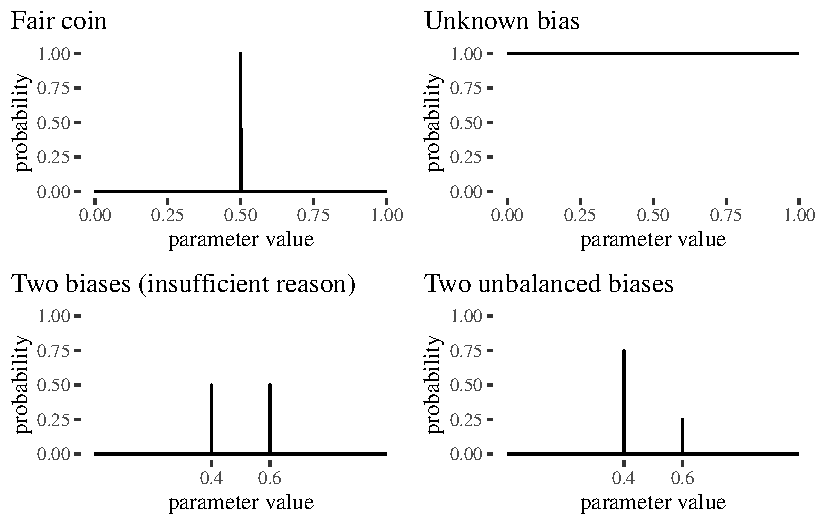
\includegraphics[width=0.8\textwidth,height=\textheight]{imp_philosophical_files/figure-pdf/fig-evidenceResponse-1.pdf}

}

\caption{\label{fig-evidenceResponse}Examples of higher-order
distributions for a few scenarios problematic for both precise and
imprecise probabilism.}

\end{figure}

An agent's uncertainty could---perhaps, should---sometimes be
represented by a sigle probability value. Higher-order probabilism does
not prohibit that. For example, there may well be cases in which an
agent's uncertainty is aptly represented by the expectation.\footnote{The
  expectation is usually defined as \(\int_{0}^{1} x f(x) \, dx\). In
  the context of our approach here, \(x\) is the first-order probability
  of a given proposition, and \(f\) is the density representing the
  agent's uncertainty about \(x\).} But this need not always be the
case. If the probability distribution is not sufficiently concentrated
around a single value, a one-point summary will fail to do justice to
the nuances of the agent's credal state.\footnote{This approach lines up
  with common practice in Bayesian statistics, where the primary role of
  uncertainty representation is assigned to the whole distribution.
  Summaries such as the mean, mode standard deviation, mean absolute
  deviation, or highest posterior density intervals are only succinct
  ways for representing the uncertainty of a given scenario.} For
example, consider again the scenario in which the agent knows that the
bias of the coin is either .4 or .6 but the former is three times more
likely. Representing the agent's credal state with the expectation
\(\mathsf{P}(X) = .75 \times .4 + .25 \times .6 = .45\) would fail to
capture the agent's different epistemic attitudes towards the two
biases. The agent believes the two biases have different probabilities,
but is also certain the bias is \emph{not} .45.

Besides its greater expressive power in modelling uncertainty,
higher-order probabilism does not fall prey to belief inertia or the
impossibility of proper scoring rules. Consider a situation in which you
have no idea about the bias of a coin. You start with a uniform
distribution over \([0,1]\) as your prior. Observing any non-zero number
of heads will exclude 0 and observing any non-zero number of tails will
exclude 1 from the basis of the posterior. The posterior distribution
will become more centered as the observations come in. This result is a
straightforward application of Bayesian updating. Instead of plugging
sharp probability values into the formula for Bayes's theorem , the
factors to be mutiplied in the theorem will be probability densities (or
ratios of densities as needed). Figure~\ref{fig-intertia2}
illustrates---starting with a uniform prior distribution---how the
posterior (beta) distribution changes after successive observations of
heads, heads again, and then tails.\footnote{Assuming independence and
  constant probability for all the observations, learning is modeled the
  Bayesian way. You start with some prior density \(p\) over the
  parameter values. If you start with complete lack of information,
  \(p\) should be uniform. Then, you observe the data \(D\) which is the
  number of successes \(s\) in a certain number of observations \(n\).
  For each particular possible value \(\theta\) of the parameter, the
  probability of \(D\) conditional on \(\theta\) follows the binomial
  distribution. The probability of \(D\) is obtained by integration.
  That is: \begin{align*}
  p(\theta \vert D) & = \frac{p(D\vert \theta)p(\theta)}{p(D)}\\
  & = \frac{\theta^s (1-\theta)^{(n - s)}p(\theta)}{\int (\theta')^s (1-\theta')^{(n - s)}p(\theta')\,\, d\theta'}.
  \end{align*}}

\begin{figure}

{\centering 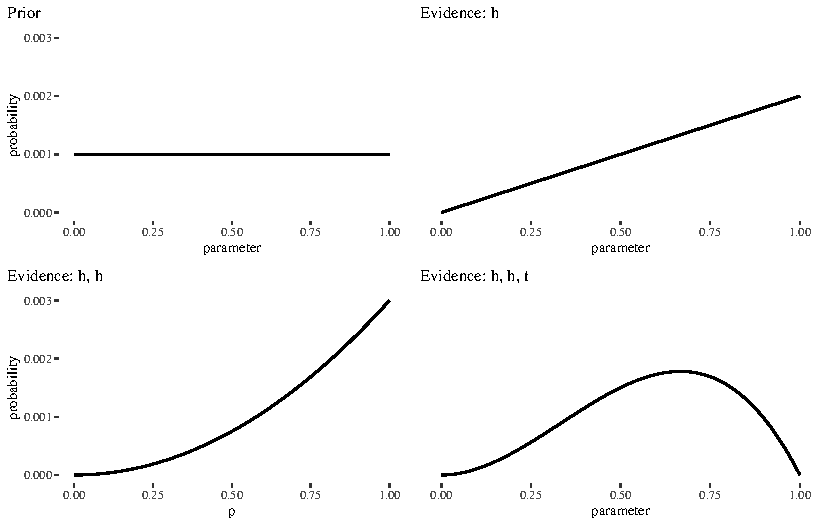
\includegraphics[width=0.8\textwidth,height=\textheight]{imp_philosophical_files/figure-pdf/fig-intertia2-1.pdf}

}

\caption{\label{fig-intertia2}As observations of heads, heads and tails
come in, extreme parameter values drop out of the picture and the
posterior is shaped by the evidence.}

\end{figure}

The impossibility of defining proper scoring rules was another weakness
of imprecise probabilism. This is a significant shortcoming, especially
because proper scores do exist for precise probabilism. Fortunately, one
can show that there exist proper scoring rules for higher-order
probabilism. These rules can then be used to formulate accuracy-based
arguments. In addition, recall the point made by Schoenfield (2017): an
accuracy measure will not usually recommend an imprecise stance. This
argument fails against imprecise probabilism: there are cases in which
accuracy considerations recommend an imprecise stance (that is, a
multi-modal distribution) over a precise one. We will defend these
claims in the next section. The argument, however, will be more formal
and a bit rough going. The section can be skipped upon first reading
without losing track of the main line of the argument.

\hypertarget{proper-scoring-for-higher-order-probabilism}{%
\section{Proper scoring for higher-order
probabilism}\label{proper-scoring-for-higher-order-probabilism}}

\label{sec:proper-scores}

A scoring rule or inaccuracy score quantifies the distance (inaccuracy)
between a probability distribution and the true state of the world. A
desirable property that any such score should have is strict propriety.
In the precise case, let \(I(p, w)\) be an inaccuracy score of a
probability distribution \(p\) relative to the true state \(w \in W\).
The score \(I(p, w)\) is strictly proper if, for any other probability
distribution \(q\) different from \(p\), the following holds:

\[\sum_{w\in W} p(w)I(p, w)< \sum_{w\in W} q(w)I(p, w).\]

\noindent  That is, the expected inaccuracy of \(p\) from the
perspective of \(p\) itself shoud always be smaller than the expected
inaccuracy of \(p\) from the perspective of another distribution \(q\).
Other common requirements are that the score \(I(p, w)\) should be a
function of the probability distribution \(p\) and the true state \(w\)
(extensionality), and that the score should be a continous function
around \(p\) (continuity). Well-known results demonstrate that the Brier
score is an extensional score for precise probabilities that is both
proper and
continous.\footnote{The Brier score is defined as the squared distance
  between the true state and the probability forecast, or formally,
  \((p(x)-V(x, w))^2\), where \(p(x)\) is the probability forecast and
  \(V(x, w)\) determines if a proposition obtains at \(w\)
  (\(V(x, w)=1\)) or not (\(V(x, w)=0\)). If, for example, the
  proposition `rain' obtains at \(w\), the forecast `rain with .9
  probability' would be more accurate at \(w\) than the forecast `rain
  with .8 probability'. If, on the other hand, the proposition `not
  rain' obtained at \(w\), the latter forecast would be more accurate.}\todo{Is the formal statement of Brier score in the footnote correct?}

Can similar results be established for imprecise probabilities? The
answer is likely to be negative, since several hurdles exist. First, a
plausible scoring rule for imprecise probabilities cannot be easily
found. Suppose an imprecise forecast assigns the {[}.8, .9{]} interval
to the outcome that it would rain tomorrow, where the true state is
`rain'. Would the {[}.6, .99{]} interval be more accurate since its .99
upper bound is closer to the true state? Intuitively, the {[}.6, .99{]}
interval should not be more accurate, otherwise the trivial interval
{[}0, 1{]} would always be more accurate than any other
interval.\footnote{To remedy this problem, a plausible inaccuracy score
  for imprecise probabilities could depend on two things: first, it
  decreases with the Brier score computed using the side of the interval
  closer to the true state; and second, the inaccuracy score increases
  with the size of the interval itself. This would block the result that
  the {[}0, 1{]} interval is always the most accurate. For more details,
  see Seidenfeld et al. (2012).} In addition, no matter how the score
for imprecise probabilities is defined, a second hurdle remains. Recall
that the notion of expected inaccuracy is needed to establish strict
propriety. Unfortunately, expected inaccuracy cannot be easily defined
for imprecise probabilities, and if it is defined, it likely leads to a
failure of propriety. To see why, let \(I([p_-, p_+], w)\) be an
inaccuracy score for the interval \([p_-, p_+]\). What is its expected
inaccuracy from the perspective of the interval \([p_-, p_+]\) itself,
or from the perspective of another interval \([q_-, q_+]\)? There is no
standard answer to this question. After all, \(I([p_-, p_+], w)\) cannot
be multiplied by \([p_-, p_+]\), in the way in which \(I(p, w)\) can be
multipled by \(p(w)\). One option is to evaluate the expected inaccuracy
of \([p_-, p_+]\) from the perspective of precise probabilities such as
\(p_-\) or \(p_+\).\footnote{So the expected inaccuracy of
  \(I_w([p_-, p_+])\) would equal
  \(\sum_{w\in W} p_-(w)I([p_-, p_+], w)\) or
  \(\sum_{w\in W} p_+(w)I([p_-, p_+], w)\).} But the impreciser would
now face a problem. If the expected inaccuracy of the interval
\([p_-, p_+]\) is evaluated from the perspective of the precise
probabilities \(p_-\) or \(p_+\), finding a proper inaccuracy score that
is also continous turns out to be impossible (Seidenfeld et al., 2012).
If, instead, the notion of expected inaccuracy is not defined, the
question whether an imprecise inaccuracy score can be proper is
ill-defined.

Despite the difficulties that plague imprecise probabilism in defining
scoring rules that are proper, here we show that there is a intuitively
plausible scoring rule for higher-order probabilities that is both
proper and continous. Building on existing work on this topic (Hersbach
(2000), Pettigrew (2012), Gneiting \& Raftery (2007)), the higher-order
scoring rule we propose is based on well-known measures of divergence
between probability distributions. In particular, we rely on the
Kullback-Leibler (KL) divergence, which is defined as follows:

\[ D_{\text{KL}}(q \,||\, p) = \sum_{x} q(x) \log\left(\frac{q(x)}{p(x)}\right) \]

\noindent This is a standard information-theoretic measure of divergence
of \(p\) from \(q\) from the perspective of \(q\). For computational
ease, we are using a grid approximation instead of continous
distribitions, as in practice we are unable to work with infinite
precision.\footnote{In the continuous case, we would need to use the so-called differential KL divergence, but our main points wouldn't change otherwise.}
To this end, \(x\) will denote the finite vector of discrete outcomes
under consideration.

The goal is to deploy KL divergence as a measure of inaccuracy of \(p\)
relative to a true state \(w\in W\), denoted by \(I_{KL}(p, w)\). To
this end, let the probability distribution \(q(x)\) play the role of the
ominiscient distribution tracking the true state \(w\), call it
\(t_w(x)\). For a possible outcome \(x\) at state \(w\), the ominscient
distribution \(t_w(x)\) will either assign probability 1 (if the outcome
obtains in \(w\)) or 0 (if the outcome does not obtain in \(w\)). Since
\(t_w(x)\) will equal one for the true outcome \(x\), call it \(x_w\),
and zero for the others, KL divergence simplifies to:
\todo{!please check that notation is correct throughout!}

\[ I_{KL}(p, w) = D_{\text{KL}}(t_w \,||\, p) = \sum_{x} t_w(x) \log\left(\frac{t_w(x)}{p(x)}\right) = \log\left(\frac{1}{p(x_w)}\right)= -\log p(x_w) \]

\noindent That is, \(I_{KL}(p, w)\) is the KL divergence of \(p\) from
the omniscient probability distribution \(t_w\).

This inaccuracy score applies to any probability distribution \(p\),
including higher-order ones. For suppose the possible outcomes are the
chance hypotheses \(\theta_1, \theta_2, \dots, \theta_n\) about the true
bias of a coin. Let \(\theta_w\) be the true bias of the coin at \(w\),
and let \(p(\theta_w)\) be the higher-order probability that the
distribution \(p\) assigns to the bias \(\theta_w\). Then,
\(-\log p(\theta_w)\) is the KL-based inaccuracy score of the
higher-order probability \(p\) at \(w\). If, for example, the true bias
of the coin is \(.6\) and the higher-order distribution \(p\) assigns
\(.8\) to this bias, the higher-order inaccuracy score of \(p\) would be
\(-\log .8\). Notice that, on this approach, two distributions \(p\) and
\(q\) which assigns the same probability to the true chance hypothesis
in \(w\)---\(p(\theta_w)=q(\theta_w)\)---will have the same inaccuracy
score \(I_{KL}\) even though they might different in the probabilities
they assign to other chance hyptheses. So the shape of the distribution
does not matter for the inaccuracy score; it does matter for expected
inaccuracy, as we will now see.

To establish the strict propriety of the scoring rule \(I_{KL}\), let's
first define the score's expected inaccuracy. If \(I_{KL}(p, w)\) is the
inaccuracy score of the distribution \(p\) at \(w\), what is its
expected inaccuracy from the perspective of the distribution \(q\)? To
this end, consider \(n\) potential true outcomes \(x_w\), each
associated with a true state \(w\) (say, \(n\) true chance hypotheses
\(\theta_w\)); then, compute the inaccuracy scores of \(p\) with respect
to each of the \(x_w\)'s (or omniscient distributions), that is,
\(-\log p(x_w)\); finally, calculate the expected inaccuracy by summing
over the entire distribution \(q\). So the expected inaccuracy is
defined as follows:

\[\sum_{w\in W} q(x_w)I_{KL}(p, w) = \sum_{w\in W} q(x_w)(-\log p(x_w)) \]

\noindent To show strict propriety, it is enough to notice two facts.
First, the expected inaccurracy of \(p\) from the perspective of \(p\)
itself is the entropy of \(p\), namely \(H(p)\).\footnote{\(\sum_{w\in W} p(x_w)I_{KL}(p, w) = -\sum_{w\in W} p(x_w)\log p(x_w) = H(p).\)}
Second, the expected inaccuracy of \(p\) from the perspective of another
distribution \(q\) is the cross-entropy between \(p\) and \(q\), namely
\(H(p, q)\).\footnote{\(\sum_{w\in W} q(x_w)I_{KL}(p, w) = H(p, q).\)}
Since \(H(p)\) is always smaller than \(H(p, q)\) (see the appendix for
details), the inaccuracy score \(I_{KL}\) is proper.

\textbf{M's REVISIONS END HERE FOR NOW}

Let's now compare, and show on an example the difference between our
approach, which uses KL-divergence and a fairly standard approach
represented by CRPS\footnote{Note that there are no readily computable
  solutions to the integral used in the definition of CRPS, although it
  can sometimes be evaluated in closed form (Gneiting \& Raftery, 2007,
  p. 366).}. todo\{Say that it is used for example by Konek\}. We will
start by providing a definition of another inaccuracy measure,
Cramer-Von-Mises. In the discretized version, it is defined
as:\footnote{In the continuous case, this measure is defined as the area under the squared Euclidean distances between the corresponding cumulative density functions That is, $D_{CM}(p,q)  = \int_{0}^{1} \vert P(x) - Q(x)\vert^2 \, dx$. Looking at cumulative densities ensures that all densities are considered on the same scale.}
\begin{align*}
D_{\text{CM}}(p,q) & = \sum_{x} \vert P(x) - Q(x)\vert^2 
\end{align*}

\noindent where \(\mathsf{P}\) is the cumulative probability
corresponding to the probability distribution \(p\).

\noindent This inaccuracy measure can be used to define the inaccuracy
of \(p\) with respect to \(w\) as follows:

\begin{align*}
I_{\text{CRPS}}(p,w) &= \sum \vert \mathsf{P}(x) - \mathbf{ 1 }(x\geq V(w))\vert ^2 
\end{align*} \noindent where: \begin{align*}
\mathbf{ 1 }(x \geq V(w)) & = \begin{cases} 1 & \text{ if } x \geq V(w)\\
0 & \text{ o$\,$/w. }
\end{cases}
\end{align*} \noindent  Cramer-Von-Mises can also be used to define the
expected inaccuracy, analogously to the case of KL-divergence.

At this point, a friend of point estimates might insist,
\emph{but who do we have to pay attention to all these possible values, we can just run with point estimates!}
To illustrate why the move to consider values in-between without prior
integration, we will go over an example in which there are only two
possible lowe-level outcomes, \(\mathsf{tails}\) and \(\mathsf{heads}\),
*and we take the distribution's expected values as the probabilities
they assign to those outcomes. On this approach, instead of calculating
inaccuracy w.r.t. to all possible hypotheses about the coin's bias, we
first average out, and proceed in terms of probabilities of the two
outcomes only instead. That is, we use:

\[\mathbb{E_{binary}}(p,q) = I(p,\mathsf{heads}) \mathbb{E}q(\mathsf{heads}) + I(p,\mathsf{tails}) \mathbb{E}q(\mathsf{tails}).\]

We will start by reflecting on this binary approach, but we will soon
see that it runs into difficulties. To fix ideas, consider a variation
of a scenario by Schoenfield (2017). A rational agent is invited to
engage in a bet by an opponent who has a representative bag of coins
coming from a factory where the distribution of bias among the coins
produced, the true generative process, is known. It is a mixture of two
normal distributions centered at \(.3\) and at \(.5\), both with
standard deviation of \(.05\). The opponent randomly selects one of
these coins and flips it. The rational agent knows all the details of
this set-up.

What credal state should the rational agent form in response? Consider
three out of many possible options: first, a \emph{faithful bimodal}
distribution centered at \(.3\) and \(.5\); second, a \emph{unimodal}
distribution centered at \(.4\); third, a \emph{wide bimodal}
distribution centered at \(.2\) and \(.6\). The three options are
depicted in Figure~\ref{fig-emc}. All of them have expected values at .4
rounded to four digits.

Denote these distributions as \(b, c,\) and \(w\) correspondingly. Now
consider what happens if we think of expected inaccuracy of these
distributions assuming there are only two possible true outcomes,
conceptualized as either heads (\(H\)) or tails (\(T\)). Whatever our
inaccuracy measure, we will have six inaccuracy scores of the form
\(I(\mathsf{distribution}, \mathsf{outcome})\), where
\(\mathsf{outcome}\) is one of two omniscient distributions that give
all weight to either heads or tails. In the calculation of expected
values,these will need to be multiplied by the probability of \(H\) and
the probability of \(T\). However, none of these distributions assigns
such a probability. They all assign probabilities to different values of
coin bias, but not to different \emph{outcomes} directly. Suppose we do
what seems to be the natural way to go for the friends of point
estimation and obtain such probabilities by taking expected values of
the form
\(\mathbb{E}_{\mathsf{distribution}}(H) = \sum (x * \mathsf{distribution}(x))\),
where \(x\) are the values on the discretized grid (as in our example
these expectations are pretty much the same, we can simply take
\(\mathsf{distribution}(H)\) to be .4):

\begin{figure}[H]

{\centering 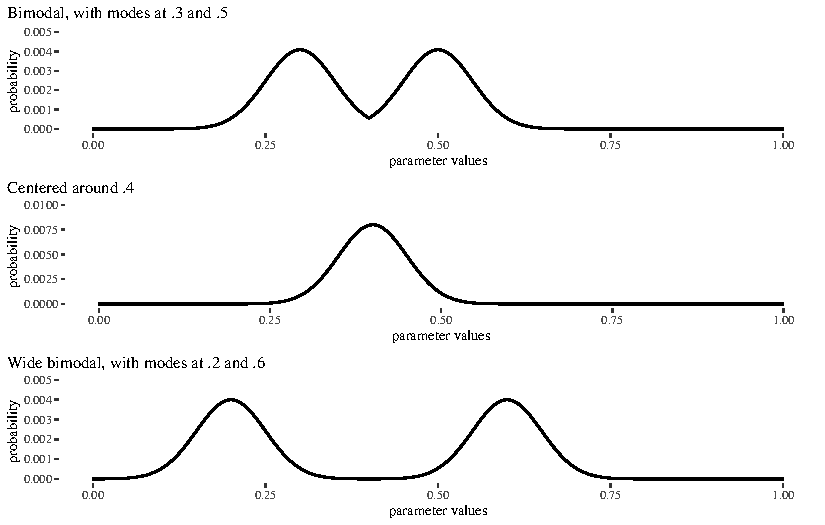
\includegraphics[width=1\textwidth,height=\textheight]{imp_philosophical_files/figure-pdf/fig-emc-1.pdf}

}

\caption{\label{fig-emc}Three distributions in a vague EMS scenario. The
distributions are built from normal distributions with standard
deviation \(.05\), the bimodal ones are joint in the middle. All of them
have expected values \(\approx .4\).}

\end{figure}

\noindent  Table \ref{tbl:comp1} displays the accuracy scores assigned
by CRPS assuming the true outcome is \emph{heads} (CRPS1) and assuming
the true outcome is \emph{tails} (CRPS0), and analogously for the KL
divergence. Then, we obtain the expected inaccuracies by averaging the
two scores by using the point probability of heads set to \(.4\). These
result in ExpCRPS and ExpKL respectively, note that since the
probability of heads is the same on all the distributions, those are
expected values from the perspective of each of the measures; changing
the perspective in this example doesn't change the expected inaccuracy.

\begin{table}[H]
\centering
\begin{tabular}{lrrrrrr}
\toprule
distribution & CRPS1 & CRPS0 & KLD1 & KLD0 & ExpCRPS & ExpKLD\\
\midrule
bimodal & 534.7305 & 334.9305 & 80.06971 & 33.90347 & 414.8505 & 52.36997\\
centered & 571.2192 & 371.4192 & 110.84220 & 53.13440 & 451.3392 & 76.21752\\
wide bimodal & 485.4052 & 285.6177 & 54.13433 & 19.50965 & 365.5340 & 33.35974\\
\bottomrule
\end{tabular}
\caption{CPRS and KLD inaccuracies of the three distributions to the TRUE and FALSE omniscient functions, with expected inaccuracies, calculated using the shared point estimates of the probabilities of heads and tails.}
\label{tbl:comp1}
\end{table}

As it turns out, the expected CRPS score recommends the wide bimodal
distribution as the most accurate (or least inaccurate). The KL
divergence from the omniscient measure makes the same
reccomendation.\footnote{This indicates that the choice of the
  evaluation metric is not the cause of the recommendation.} This is
counterintuitive, because the faithful bimodal seems the one most
appropriately evidence-responsive. The unimodal distribution, while
centering on the expected value, gets the chances wrong, and the wide
bimodal has its guesses too close to the truth values and too far from
the known chances. But there is a further problem. While the wide
bimodal distribution expects itself to be the least inaccurate, the
other distributions also expect the wide bimodal to be the least
inaccurate. This indicates that in this setting the CRPS score and the
KL divergence are not proper scores, as they allow for cases of some
distributions recommending other distributions as less accurate,
whatever the true state of the world turns out to be.

What are we to make of this result? Note that the three distributions
share the same expected value \(.4\). The latter is then used in the
calculations of the expected inaccuracies for both CRPS and KL with the
assumption there are two possible outcomes with respect to which
expected inaccuracy calculations are to be made. This approach, however,
runs against the spirit of our enterprise. If expected values are often
not good representations of a rational agent's uncertainty, it should
not be surprising that relying on them fails to deliver plausible
expected accuracy scores. By reducing each of the distributions' stance
towards heads to a single point value .4, we've effectively washed out
key information. So the question is, how can we adequately account for
the complexity of a rational agent's credal state in formulating a
proper accuracy score?

Our proposal is that rather than measuring inaccuracy in relation to
``true states of the world'' conceptualized as two omniscient credences
that peak at either 0 or 1 and averaging using expected values of the
distributions, we should instead utilize a set of \(n\) potential true
probability hypotheses (ideally, going continuous, but we're working
with a discrete grid of \(n=1000\) possible coin baises in this paper).
We then compute all the inaccuracies with respect to each of these \(n\)
values represented by ``omniscient'' distributions (or true chance
hypotheses) and determine the expected inaccuracy scores using the
entire distributions rather than relying solely on the expected values
of the distributions.

For the three distributions under consideration, the accuracy scores
calculated using CRPS and KL divergence with respect to omniscient
distributions corresponding to various values of \(x\) are given by
Figure~\ref{fig-inaccuracies2}. The expected inaccuracies of the
distributions from their perspective are given by
\mbox{Table \ref{tbl:expected2}.} The results now match our common
sense: each distribution recommends itself. So, once we pay attention to
the whole range of possiblities, the CRPS score and KL divergence are
now proper scores.

\begin{figure}[H]

{\centering 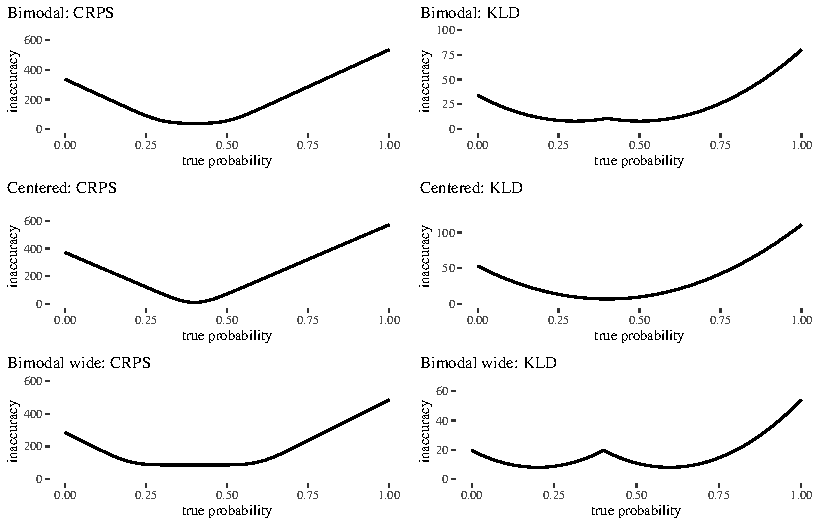
\includegraphics[width=1\textwidth,height=\textheight]{imp_philosophical_files/figure-pdf/fig-inaccuracies2-1.pdf}

}

\caption{\label{fig-inaccuracies2}CLPSR and KL divergence based
inaccuracies vs (omniscient functions corresponding to) \(n\) true
probability hypotheses for the three distributions discussed in this
section.}

\end{figure}

\begin{table}[H]
\begin{tabular}{lrrrrrr}
& \multicolumn{3}{c}{CPRS} & \multicolumn{3}{c}{KLD} \\
\toprule
  & bimodal & centered & wide bimodal & bimodal & centered & wide bimodal\\
\midrule
bimodal & 64.670 & 78.145 & 88.380 & 8.577 & 10.655 & 11.336\\
centered & 41.657 & 28.181 & 85.911 & 9.239 & 7.690 & 15.627\\
wide bimodal & 137.699 & 171.719 & 113.989 & 11.541 & 19.231 & 8.689\\
\bottomrule
\end{tabular}
\caption{Expected inaccuracies of the three distributions from their own perspectives.
 Each row corresponds to a perspective.}
\label{tbl:expected2}
\end{table}

One important difference transpires between using CRPS and KLD. Notice
how for chance hypotheses between the actual peaks the inaccuracy
remains flat. This seems to be an artifice of choosing a squared
distance metric. If instead we go with a more principled,
information-theory-inspired KL divergence, inaccuracy in fact jumps a
bit for values in between the peaks for the bimodal distributions, which
seems intuitive and desirable. This seems to be a reason to prefer a
KL-based accuracy measure.

One question remains: how does the framework capture the idea that it is
the bimodal distribution that seems more adequate than the others? One
way to interpret that is by looking at inaccuracy concerning chance
hypotheses given by the testimonial evidence. In this case, these are
\(H_3\), where the true chance is \(0.3\), and \(H_5\), where the true
chance is \(0.5\). You can find the specific inaccuracies for them in
Table \ref{tbl:schoen}. To make sure that this favorable outcome isn't
due to not using pointed credences, we can redo the calculations using
the pointed version. In the pointed version, all the focus is on 0.4, or
the weight is evenly divided between 0.3 and 0.5, or between 0.2 and
0.6. As anticipated, when we consider inaccuracy, both of these setups
recommend the bimodal version (Table \ref{tbl:schoen2}).

\begin{table}[H]
\centering
\begin{tabular}{lrrrr}
 & \multicolumn{2}{c}{CRPS} & \multicolumn{2}{c}{KLD} \\
\toprule
&H3 & H5 & H3 & H5\\
\midrule
bimodal &55.475 & 55.378 & 7.935 & 7.935\\
centered &72.281 & 72.090 & 9.836 & 9.825\\
wide bimodal & 86.230 & 86.223 & 10.871 & 10.882\\
\bottomrule
\end{tabular}
\caption{CRPS and KLD inaccuracies of the three distributions with respect to the two hypotheses. On both inaccuracy measures the bimodal distribution dominates the other two.}
\label{tbl:schoen}
\end{table}

\begin{table}[H]
\centering
\begin{tabular}{lrrrr}
 & \multicolumn{2}{c}{CRPS} & \multicolumn{2}{c}{KLD} \\
\toprule
 &H3 & H5 & H3 & H5\\ \midrule
pointed bimodal &49.75 & 49.75 & 1.00 & 1.00\\
pointed centered &100.00 & 100.00 & 16.61 & 16.61\\
pointed wide bimodal & 99.75 & 99.75 & 16.61 & 16.61\\
\bottomrule
\end{tabular}
\caption{CRPS and KLD inacurracies of the three-pointed distributions with respect to the two hypotheses.}
\label{tbl:schoen2}
\end{table}

\hypertarget{evidence-aggregation-the-simple-case}{%
\section{Evidence aggregation: the simple
case}\label{evidence-aggregation-the-simple-case}}

Rational agents are often tasked with aggregating pieces of evidence and
assessing their value relative to a hypothesis. In this and the next
section, we examine the question of how multiple items of evidence
should be evaluated together. This question raises novel difficulties
for both precise and imprecise probabilism. We show how higher-order
probabilism can handle them.

For the precise probabilist, a natural measure of the value of the
evidence is the likelihood ratio. This ratio is relative to a pair of
competing hypotheses, say \(H\) and its negation \(\neg H\) (though the
two hypotheses need not be one the negation of the other). Relative to
these hypotheses, the likelihood ratio of a single piece of evidence
\(E\) is the probability of \(E\) given \(H\) divided by the probability
of \(E\) given \(\neg H\), or in short,
\(\frac{\pr{E \vert H}}{\pr{E \vert \neg H }}\). Degrees of evidential
value (or support, strength) can be expressed as follows:

\begin{quote}
the higher $\frac{\pr{E \vert H}}{\pr{E \vert \neg H }}$ (if greater than one), the more strongly $E$ supports $H$.
\end{quote}

\noindent The value of the evidence increases whenever
\(\pr{E \vert H}\) increases or whenever \(\pr{E \vert \neg H }\)
decreases. The higher \(\pr{E \vert H}\), the better the evidence at
tracking \(H\) (a true positive); the lower \(\pr{E \vert \neg H }\),
the better the evidence at avoiding \(\neg H\) (a true negative). If the
probability of \(E\) is the same given hypothesis \(H\) as given its
negation, that is, the likelihood ratio equals one, the evidence would
have no value for \(H\).

Likelihood ratios can also be used for assessing the value of multiple
pieces of evidence in the aggregate, again relative to a pair of
hypotheses of interest. In the simplest case (for more complex cases,
see the next section), multiple items of evidence all bear on the same
hypothesis. Then, to obtain their combined evidential value, it is
enough to multiply their individual likelihood ratios.

\[
\frac{\pr{E_1 \wedge E_1 \dots E_k \vert H}}{\pr{E_1 \wedge E_2 \dots E_k \vert \neg H}} = \frac{\pr{E_1 \vert H}}{\pr{E_1 \vert \neg H}}\times \frac{\pr{E_2 \vert H}}{\pr{E_2 \vert \neg H}} \times \dots \times \frac{\pr{E_k \vert H}}{\pr{E_k \vert \neg H}}
\]

\noindent The equality holds provided \(E_1, E_2, \dots, E_k\) are
probabilistically independent conditional on hypothesis \(H\) and its
negation. Think, for example, at several diagnostic tests performed by
independent laboratories or independent witnesses in a trial testifying
about the same issue.

To see how likelihood ratios can be deployed, it is worth working
through a specific case. In a murder case, the police recover two items
of trace evidence, both against the defendant. First, hair found at the
crime scene matches the defendant's hair; call this evidence
`\textsf{hair}.' Second, the fur of the defendant's dog matches the fur
found in a carpet wrapped around one of the bodies; call this evidence
`\textsf{fur}.'\footnote{The hair evidence and the dog fur evidence are
  stylized after two items of evidence in the notorious 1981 Wayne
  Williams case (Deadman, 1984b, 1984a).} The two matches favor the
hypothesis that the defendant (and the defendant's dog) must be the
source of the crime traces; call this hypothesis `\(\mathsf{source}\)'.
If the two matches are independent lines of evidence (conditional on the
source hypothesis and its negation), their likelihood ratios can be
multiplied:

\[
\frac{{\pr{\s{fur} \wedge \s{hair}  \vert \s{source}}}}{{\pr{\s{fur} \wedge \s{hair} \vert \neg \s{source}}}} = \frac{{\pr{\s{fur} \vert \s{source}}}}{{\pr{\s{fur}  \vert \neg \s{source}}}} \times
 \frac{{\pr{\s{hair} \vert \s{source}}}}{{\pr{\s{hair} \vert \neg \s{source}}}}
\]

So far so good. But how do we fill in the precise probabilies? The
numerators can be equated to one: if the defendant is a contributor, the
laboratory will declare a match for sure. This is a simplication, but it
will do for our purposes. To fill in the denominators, a trial expert
will provide so-called match probabilities. They express the likelihood
that, by coincidence, a random person (or a random dog) who is not a
contributor would still match. The match probabilities are approximated
by counting how many matches are found in a representative sample of the
human population (or the canine population). Suppose the matching hair
type occurs 0.0253 times in a reference database, and the matching dog
fur type occurs 0.0256 times in a reference database (more on how these
numbers are calculated soon). These frequencies can fill in the match
probabilities. Putting everything together: \begin{align*}
\frac{{\pr{\s{dog} \vert \s{source}}}}{{\pr{\s{dog}  \vert \neg \s{source}}}} \times
 \frac{{\pr{\s{hair} \vert \s{source}}}}{{\pr{\s{hair} \vert \neg \s{source}}}}
& =  \frac{1}{0.0252613} \times  \frac{1}{0.025641} = {1543.862069}
\end{align*}

\noindent The resulting ratio is large. The two matches, combined,
strongly favor the source hypothesis.

This is the story about evidence aggregation told by the precise
probabilist. But this story misses something crucial. As it happens, the
match probability for hair evidence is based on 29 matches found in a
sample database of size 1148, while the match probability for the dog
evidence is based on finding two matches in a smaller database of size
78. The relative frequencies are about \(.025\) in both cases, but the
two samples differ in size. The smaller the sample, the greater the
uncertainty about the match probabilities. So, for individual pieces of
evidence, simply reporting the exact numbers makes it seem as though the
evidential value of the matches is the same, but actually it is
not.\footnote{The match probabilities in the Wayne Williams case on
  which our running example is based were 1/100 for the dog fur, and
  29/1148 for Wayne Williams' hair. Match probabilities have been
  slightly but not unrealistically modified to be closer to each other
  in order to make a conceptual point: the same first-order
  probabilities, even when they sound precise, may come with different
  degrees of second-order uncertainty.} In the aggregate, multiplying
the individual likelihood ratios further washes away this difference.

A better alternative is easily available: the evaluation of multiple
items of evidence should take into account higher-order uncertainty.
Figure~\ref{fig-densities} (upper part) depicts higher-order probability
distributions of different match probabilities given the sample
data---the actual number of matches found in the sample databases. As
expected, some random match probabilities are more likely than others,
and since the sizes of the two databases are different, the
distributions have different spreads: the smaller the database the
greater the spread, the greater the uncertainty about the match
probability. In light of this, Figure~\ref{fig-densities} (lower part)
depicts the probability distribution for the joint match probability
associated with both items of match evidence, hair and fur evidence. The
aggregate value of the two pieces of match evidence, then, is given by a
distribution over possible likelihood ratios.
\todo{add distributions of LRs figure} The shape of this distribution
conveys the degree of higher-order uncertainty about the value of the
aggregate evidence.
\textbf{Marcello (Rafal/Nikodem to add): Can we have a formula of how the two matches are combined in the higher-order approach? In precise probabilism, you multiply the individual LRs, in higher-order probabilism, what do we do formally? Can we also have a distribution of likelihood ratios? What happens if both numerator and denominator in the LR are distributions?}

\begin{figure}[H]

{\centering 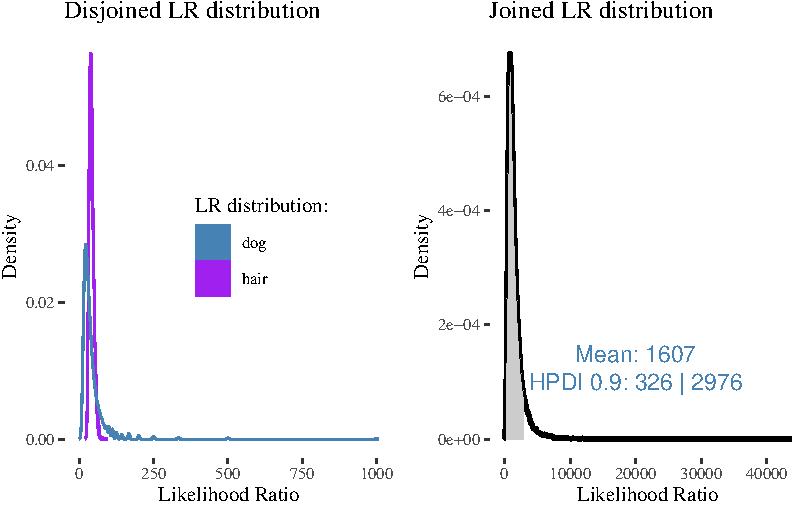
\includegraphics[width=0.9\textwidth,height=\textheight]{imp_philosophical_files/figure-pdf/fig-lrdens-1.pdf}

}

\caption{\label{fig-lrdens}Distributions of dog and hair likelihood
ratios and the resulting joint likelihood ratio. Created with the
samples from beta distributions. Shaded area on the second one
represents HPDI with 0.9 credibility.}

\end{figure}

\begin{figure}[H]

{\centering 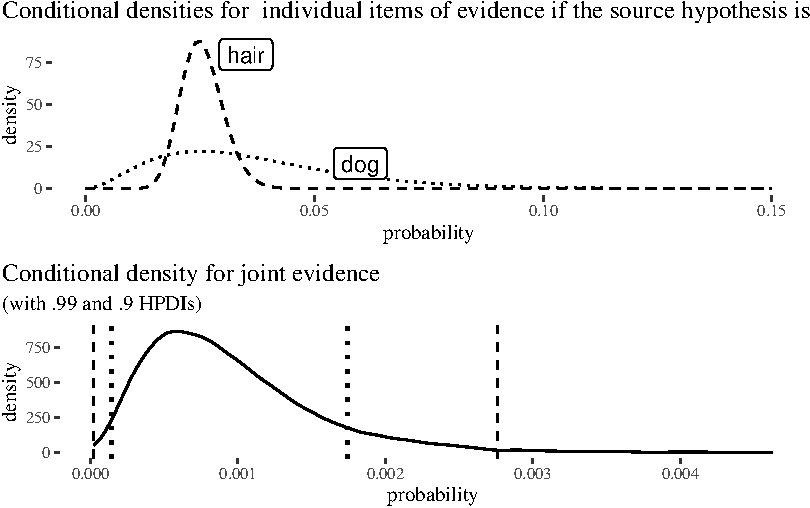
\includegraphics[width=0.8\textwidth,height=\textheight]{imp_philosophical_files/figure-pdf/fig-densities-1.pdf}

}

\caption{\label{fig-densities}Beta densities for individual items of
evidence and the resulting joint density with .99 and .9 highest
posterior density intervals, assuming the sample sizes as discussed and
independence, with uniform priors.}

\end{figure}

The precise probabilist might insist that the value of the
evidence---one item or multiple items of evidence---is naturally
captured by a precise likelihood ratio. In our running example, this
ratio equals one over the first-order match probabilty, and our best
assessment of this first-order probability is still the relative
frequency of matches found in the database, whether large or small. If
this is right, our best assessment of the match probabilities for both
fur and hair evidence should be about \(.025\), based on the relative
frequencies 2/78 and 29/1148. If we were to bet whether a dog or a human
picked at random would have the matching fur or hair type, our odds
should be \(.025\) no matter the size of the database. This argument has
some bite when evaluating single items of evidence. In fact, the
expected values of the match probabilities for hair and match
evidence---based on the higher-order distributions in
Figure~\ref{fig-densities} (upper part)---still end up being about
\(.025\). If, as the precise probabilist assumes, first-order
probabilities is all we should care about, going higher-order would seem
a needless complication.

This line of reasoning, however, breaks down when evaluating two or more
items of evidence. What should our betting odds be for the proposition
that a human and a dog, both picked at random, would have the matching
fur and hair type in question? For the precise probabilist, the answer
is straightforward: on the assumption of independence, it is enough to
multiply the \(.025\) individual match probabilities and obtain a joint
match probability of \ensuremath{6.4772626\times 10^{-4}}. The
higher-order probabilist will proceed differently. In assessing
first-order match probabilities, they will retain information about
higher-order uncertainty as much as possible. This can done in two
steps: first, aggregate the higher-order distributions for the two match
probabilities and obtain a higher-order probability distribution for the
joint match probability (see Figure~\ref{fig-densities}); next, to
obtain our best assessment of the first-order joint match probability,
take the expected value of this latter distribution. The higher-order
probabilist will assign \ensuremath{9.381365\times 10^{-4}} to the joint
match probability, a value greater than what the precise probabilist
would assign.

So, the higher-order and precise probabilist will disagree about the
betting odds for the proposition that a human and a dog, both picked at
random, would have the matching fur and hair type. The disagreement will
become even starker as a larger number of independent items of evidence
are evaluated.\footnote{Consider the simple case of independent items of
  evidence whose individual match probabilities are \(.025\). For three,
  five and seven items of evidence, the joint match probabilities would
  be: \ensuremath{1.25\times 10^{-4}},\ensuremath{3.125\times 10^{-7}}
  and \ensuremath{7.8125\times 10^{-10}} (for the precise probabilist)
  and \ensuremath{5.3363868\times 10^{-4}},
  \ensuremath{1.6754185\times 10^{-5}} and
  \ensuremath{9.9986742\times 10^{-7}} (for the higher-order
  probabilist, based on small databases of size 20).} Who should be
trusted? Since the higher-order probabilist takes into accout more
information---that is, the higher-distributions---there is good reason
to think that the higher-order probabilist should be trusted more than
the precise probabilist.\footnote{As a further illustration of this
  point, consider a couple of variations of our running example. First,
  suppose the match probabilities associated with two matches are both
  set to \(.05\), since they are based on the following relative
  frequencies: one match occurs in a dog fur database and one match
  occurs in a human hair database, where both databases are small, say
  of size 20. By multiplying the individual \(1/.05\) likelihood ratios
  associated with the two matches, their evidential value against the
  defendant would seem quite strong: \(1/.05\times 1/.05=400\). But the
  match probabilities are based on frequencies resulting from small
  databases, so their evidential value should be rather weak. Precise
  probability here seems to exaggerate the aggregate value of the
  evidence. Following higher-order probabilism, the joint likelihood
  ratio would be 237.8675988, a significantly smaller value. On the
  other hand, if the same \(.05\) match probabilities were based on
  larger databases, the evidential value of the two matches should be
  correspondingly greater, but precise probabilism would make no
  difference. If, for example, 1,000 hair and fur matches are found in
  databases of size 20,000, the higher-order probabilist would assign
  441.2059925 to the joint likelihood ratio, a much greater value than
  before. This outcome agrees with our intuituions.}

Imprecise probabilism will also run into its own problems when assessing
the value of aggregate evidence. Recall that the probability measures in
the representor set are those compatible with the evidence. The problem
is that almost any random match probability will be compatible with any
sample data---with any number of matches found in a reference database.
This point should be familiar from the earlier discussion. Think by
analogy to coin tossing: even a coin that has a .99 bias toward tails
could come up heads on every toss. This series of outcomes is unlikely,
but possible. Similarly, a hair type that has a match probability
extremely small could still be found several times in a sample
population. So, it is not clear how to proceed if one takes seriously
the binary notion of compatibility. Imprecise probabilism is too
permissive because almost any match probability will be compatible with
the data.

Another option for the imprecise probabilist is to rely on reasonable
ranges of match probabilities. Suppose these ranges are (.015,.037)
(.002, .103), for hair and fur evidence respectively in our original
case.\footnote{These are 99\% credible intervals starting with uniform
  priors. A 99\% credible interval is the narrowest interval to which
  the expert thinks the true parameter belongs with probability .99. For
  a discussion of what credible intervals are, how they differ from
  confidence intervals, and why confidence intervals should not be used,
  see Kruschke (2015).} As expected, the range is wider for dog fur
match evidence than hair match evidence: the uncertainty about the dog
fur match probability is greater since the sample database was smaller.
This is a desirable feature of the interval approach. Now, to assess the
joint uncertainty, it is enough to focus on what happens at the edges of
the two intervals. Reasoning with representor members at the edges of
the intervals will yield the most extreme probability measure the
impreciser is committed to, the worst-case and best-case scenarios. We
end up with a new range for the joint match probabilties, (.00003,
.003811).\footnote{Redoing the calculations using the upper bounds of the two intervals, $.037$ and $.103$,  yields the following:
\begin{align*}
\mathsf{P}(\s{dog}\wedge \s{hair} \vert \neg \s{source})   & =  .037 \times .103 =.003811.
\end{align*}

\noindent
 This number is around 5.88 times greater than the original estimate. Given this number, the two matchs are much weaker evidence for the source hypothesis than previously thought.    The calculation for the lower bounds, $.015$ and $.002$, yields the following:
\begin{align*}
\mathsf{P}(\s{dog}\wedge \s{hair} \vert \neg \s{source})   & =  .015 \times .002 =.00003
\end{align*}
   
 \noindent  
This number is around 0.46 times lower than the original estimate.  Given this number, the two matchs are much stronger evidence for the source hypothesis than previously thought.}
The corresponding likelihood ratios could be as high as
\ensuremath{3.3333333\times 10^{4}} or as low as 262.3983. The two
matches could be much stronger or much weaker evidence than previously
thought.

Using plausible ranges for the match probabilities leaves the impression
that any value in the interval is just as good as any other. Perhaps we
should pick the middle value as representative of the interval. However,
relying on the entire interval or the middle value will misrepresent the
evidence. To see why, consider again Figure~\ref{fig-densities} (lower
part) which depicts the probability distribution for the joint match
probability. Interestingly, this distribution is not symmetric. So the
most likely value (and the bulk of the distribution, really) does not
lie in the middle between the edges. Therefore, only relying on the
edges---or taking central values as representative of the interval---can
lead to overestimating or underestimating the probabilities at
play.\footnote{The calculations for the joint interval assume that because the worst- or best-case probability for one event is $x$ and the worst- or best-case probability for another independent event is $y$, the worst- or best-case probability for their conjunction is  $xy$. However, this conclusion does not follow if the margin of error (credible interval) is fixed. Just because the probability of an extreme value $x$ for one variable $X$ is .01, and so it is for the value $y$ of another independent variable $Y$, it does not follow that the probability that those two independent variables take values $x$ and $y$ simultaneously is the same. In general, it is impossible to calculate the credible interval for the joint distribution based solely on the individual credible intervals corresponding to the individual events.}

Another problem in taking intervals as representative of the value of
the evidence is that they will tend to widen as more items of evidence
are evaluated. The size of the likelihood ratio interval was initially
39.64 (hair evidence) and 490.29 (fur evidence). After aggregating the
two items of evidence, the likelihood ratio interval widened to
\ensuremath{3.3070935\times 10^{4}}. The size of the match probability
interval was initially -0.022 (hair evidence) and -0.101 (fur evidence).
After aggregating the two items of evidence, the match probability
interval narrowed to -0.003781. Posterior interval (starting with 1:1
prior odds) was initially 0.0209015 (hair evidence) and 0.0913857 (fur
evidence). After aggregating the two items of evidence, the posterior
interval narrowed to 0.0037665.

\todo{LR intervals widen but match and posterior probability intervals do not? How does that work? How can we claim that uncertainty increases?}

All in all, precise and imprecise probabilism do not fare well in
modelling the value of evidence in the aggregate. Instead, the
evaluation of multiple items of evidence should take into account
higher-order uncertainty (as illustrated in Figure~\ref{fig-densities}).
Whenever probability distributions for the probabilities of interest are
available (and they should be available for match evidence and many
forms of scientific evidence whose reliability has been studied), those
distributions should be reported for assessing the value of the
evidence. This approach avoids hiding actual aleatory uncertainties
under the carpet. It also allows for a more balanced assessment of the
evidence, whereas using point values or intervals may exaggerate or
underestimate the value of the evidence.

A couple of clarifications are in order. First, the problem we are
highlighting is not confined to match evidence. Say an eyewitness
testifies against the defendant: they saw the defendant near the crime
scene at the relevant time. To assess the value of this testimony, one
should know something analogous to the match probability: if the
defendant was not there, how probable is it that the witness would still
say the defendant was there? Or suppose a medical test for a disease
turns out positive. Here again, to asses the evidential value of the
positive test, one should know how probable it is that the test would
still turn out positive even when a patient is actually negative. And so
on. These false positive probabilities are usually derived from
sample-based frequencies in surveys or experiments: how often witness
misidentify people; how often tests misdiagnose; etc. So, depending on
the sample size, the false positive probabilities will have different
degrees of uncertainty, and the latter should be taken into account when
evaluating eyewitness testimonies, diagnostic test results, and many
other forms of evidence. At the same time---and this is the second
clarification---this discussion is not meant to suggest that the problem
we are highlighting is confined to differences in sample size; it is
broader than that. Probabilities can be subject to uncertainty for other
reasons, for example, when they are derived from a probability model for
which there is little support, or when the sample size is large but
unrepresentative. So, in short, the problem of higher-order uncertainty
is widespread and goes beyond match evidence and questions of sample
size.

\hypertarget{evidence-aggregation-the-complex-case}{%
\section{Evidence aggregation: the complex
case}\label{evidence-aggregation-the-complex-case}}

We looked at simples case of evidence aggregation: the pieces of
evidence were about the same hypothesis and probabilistically
independent. But different pieces of evidence can bear on different
hypotheses and be probabilistically dependent. Think, for example, of
two witnesses testifying in a trial about two related issues, say the
defendant's whereabouts and the defendant's motive. In these more
complex cases, precise probabilism handles evidence aggregation with the
help of Bayesian networks. The grahical part of a Bayesian nextwork
consists of nodes and arrows. Arrows between nodes visually represents
relationships of probabilistic dependencd between different hypotheses
and items of evidence, each corresponding to a node in the network. The
numerical part of a Bayesian network describes the strenghts of these
dependencies. On a purely formal level, the numerical part consists of
probability tables that are filled in with precise prior probabilities
(for nodes without incoming arrows) or conditional probabilities (for
nodes with incoming arrows).\footnote{The simple case considered in the
  previous section would consist of a network with \(k+1\) nodes, with a
  root node for the hypothesis \(H\) and then \(k\) arrows going from
  \(H\) node to the evidence nodes \(E_1, E_2, \dots, E_k\). The
  probability tables would be filled in with prior probabilities for
  \(H\) and conditional probabilities \(\pr{E_i \vert H}\) and
  \(\pr{E_i \vert \neg H}\), for any item of evidence \(E_i\). Notice
  that these conditional probabilities are those occuring in the
  individual likelihood ratios
  \(\frac{\pr{E_1 \vert H}}{\pr{E_1\vert \neg H}}\). There is no need to
  rely on a Bayesian network in such a simple case because the
  dependencies between nodes are limited.} Equipped with these input
probabilities, the network can run the calculations about the output
probabilities of interest.\footnote{The calculations can quickly get out
  of hand, so softwares exist to perform the calculations automatically.}
We might be interested, for example, in the probability of a hypothesis
given several items of evidence, while keeping track of dependencies
between them. In the standard formulation, Bayesian networks run on
precise probabilities, but can be extended to handle imprecise and
higher order-probabilities. This is the topic of this section.

As an illustration, let us start with a Bayesian network developed by
Fenton \& Neil (2018).
\todo{Why is a node for death is missing in the network? That seems necessary as parte of the evidence, no?}The
network in Figure \ref{fig-scbnplot} represents the key items of
evidence in the infamous British case R. v. Clark (EWCA Crim 54, 2000).
Sally Clark, mother of two sons, witnessed her first son die in 1996
soon after birth. Her second son died in similar circumstances a few
years later in 1998. These two consecutive deaths raised suspicion. One
hypothesis about the cause of death is that Sally murdered her children.
An alternative explanation is that both children died of Sudden Infant
Death Syndrome (SIDS). At trial, however, the pediatrician Roy Meadow
testified that the probability that a child from a family like the
Clark's would die of SIDS was quite low, 1 in 8,543. Assuming
probabilistic independence between the two events, the probability of
both children dying of SIDS becomes extremely low. It equals the product
of the two probabilities, approximately 1 in 73 million. Based on this
low probability and signs of bruising on the bodies, Sally Clark was
convicted of murder. The conviction was reversed on appeal thanks to new
evidence, specifically, signs of a potentially lethal disease found in
one of the bodies.

\begin{figure}[H]

{\centering 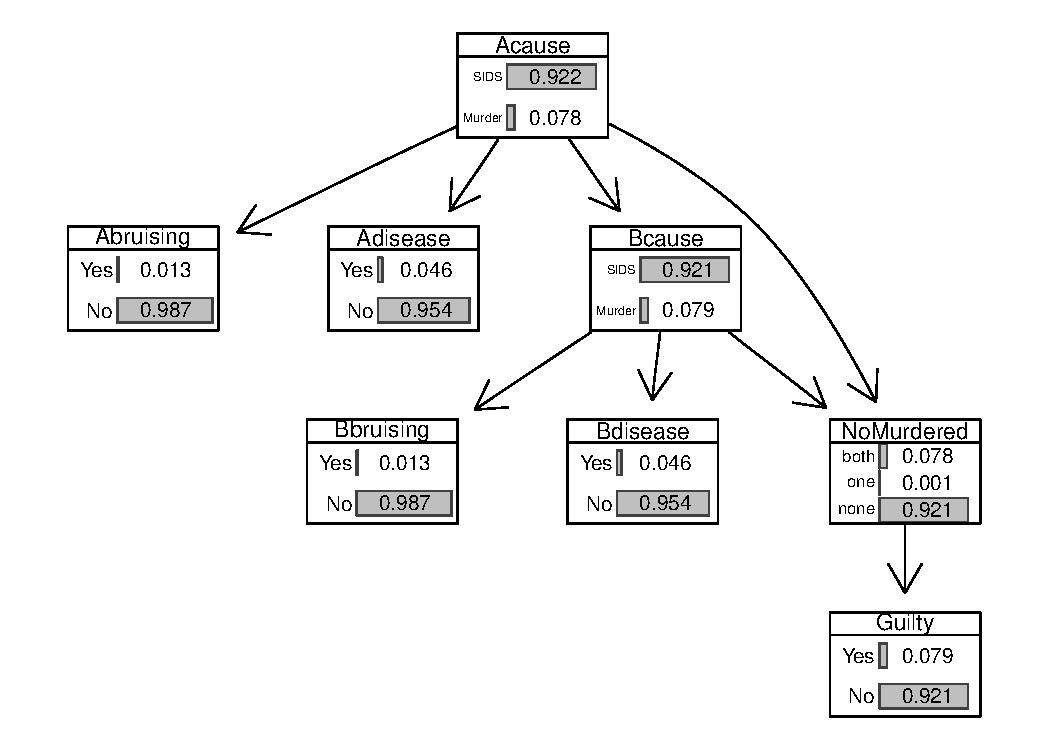
\includegraphics[width=0.8\textwidth,height=\textheight]{imp_philosophical_files/figure-pdf/fig-scbnplot-1.pdf}

}

\caption{\label{fig-scbnplot}Bayesian network for the Sally Clark case,
with marginal prior probabilities.}

\end{figure}

Much has been written about Sally Clark by philosophers and
statisticians. The discussion has often focused on whether Meadow was
allowed to assume, as he did, that the two SIDS death would be
independent events. The assumption of independence delivered the low
probability of 1 in 73 million by multiplying 1 in 8,543 by itself.
Another, much discussed point was this: even if it was unlikely that two
consecutive SIDS deaths would occur, it does not follow it was likely
that Sally murdered her children.\footnote{One could reason that, since
  1 in 73 million is a low probability, the alternative explanation,
  that Sally murdered her children, should be likely. But that a mother
  would do such a thing is also unlikely, perhaps even less likely than
  1 in 73 million.} A Bayesian network helps to avoid these mistakes. It
also help to view the case holistically. The two consecutive deaths were
an important piece of evidence, but other evidence was also important,
including signs of bruising and signs of a lethal disease as they were
discovered during the appeal process.

Unfortunately, Bayesian networks, in their standard formulation, inherit
the shortcomings of precise probabilism. The choice of the input
probabilities should be precise, and it is often unclear where the
values come from or whether they are justified. Consider, for example,
the probability that a death by SIDS would occur. How sure are we that
this probability equals, exactly, 1 in 8,543? The figure Meadow used is
a sample-based frequency. How big was that sample? How representative?
Other input probabilities need to be entered in the network to carry out
the calculations, for example, the probability that a mother would kill
her son, or the probability that signs of brusing would be found given
the hypothesis that Sally was trying to murder her child, and so on.
There will be uncertainity about these probabilites, since they are
based on sample frequencies or expert elicitation.

The standard response to these concerns is to invoke \emph{sensitivity
analysis}: a range of plausible values is tested. Say we are interested
in the output probability that Sally is guilty. The network is updated
by the known facts---the items of evidence---following standard Bayesian
conditionalization. The input probabilities in the network are then
assigned a range of possible values to see how they impact the output
probability of Sally's guilt. Sensitivity analysys is another variant,
perhaps more rudimentary, of the interval approach we considered
earlier. \todo{add references to imprecise BNs; see footnote.} In fact,
Bayesian networks for reasoning with intervals and imprecise
probabilisties already exist.\footnote{One can use uniform sampling with
  Bayesian networks to approximate the impreciser's commitments
  \textbf{Cite} \url{https://arxiv.org/abs/2302.09656}. Another approach
  is to rely on probabilistic programs with the restriction that the
  variables corresponding to probabilities are sampled from uniform
  distributions corresponding to the representor set. A critical survey
  of approaches along these lines shows that, in complex reasoning
  situations, `'the imprecision of inferences increases rapidly as new
  premises are added to an argument''.\textbf{add ref to}
  \url{https://www.sciencedirect.com/science/article/pii/S0004370296000215}.}
But, as discussed earlier, imprecise probabilism, the interval approach
and sensitivity analysis ignore the shape of the underlying
distributions. They do not distinguish between probability measures (or
point estimates) in terms of their plausibility, even though some will
be more plausible than others. Moreover, if the sensitivity analysis is
only guided by the values at the edges of the interval, these extremes
will often play an undeservedly strong role.

These concerns can be addressed by recourse to higher-order
probabilities. In a precise Bayesian network, each node is associated
with a probability table determined by a finite list of numbers (precise
probabilities). In an imprecise Bayesdian network, each node is
associated with a table dertermined by an interval of numbers. But
suppose that, instead of precise numbers or intervals of numbers, we
have distributions over the possible numbers to enter into the
probability tables.\footnote{The densities of interests can then be
  approximated by (1) sampling parameter values from the specified
  distributions, (2) plugging them into the construction of the BN, and
  (3) evaluating the probability of interest in that precise BN. The
  list of the probabilities thus obtained will approximate the density
  of interest. In what follows we will work with sample sizes of 10k.}
An example of such higher-order Bayesian network for the Sally Clark
case is represented in Figure \ref{fig-scwithhop}.

The higher-order Bayesian network helps to investigate the impact of
different items of evidence on Sally Clark's probability of guilt (see
Figure~\ref{fig-scwithhop2}). The starting point is the prior
distribution for the \s{Guilt} node (first graph). Next, the network is
updated with evidence showing signs of bruising on both children (second
graph). Next, the assumption that both children lack signs of
potentially lethal disease is added (third graph). Finally, we consider
the state of the evidence at the time of the appellate case: signs of
bruising existed on both children, but signs of lethal disease were
discovered only on the first child. Interestingly, in the strongest case
against Sally Clark (third graph), the median of the posterior
distribution is above .95, but the uncertainty around that median is
still quite wide.\footnote{The lower limit of the 89\% Highest Posterior
  Density Intervals (HPDI) is at .83.} This underscores the fact that
relying on point estimates can lead to overconfidence.

\begin{figure}[htbp] 
    \centering
    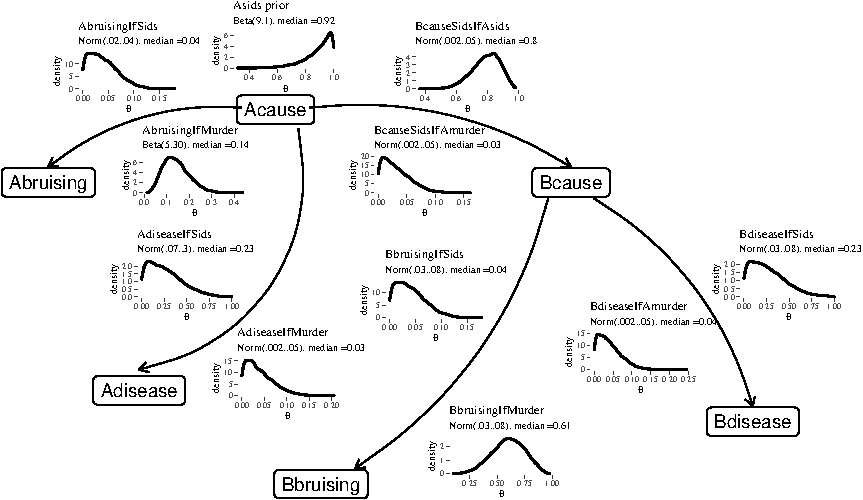
\includegraphics[angle=90, width=\textwidth]{imp_philosophical_files/figure-pdf/SCwithHOP-1.pdf}
    \caption{An illustration of a probabilistic program for the Sally Clark case.}
    \label{fig-scwithhop}
\end{figure}

\begin{figure}[H]

{\centering 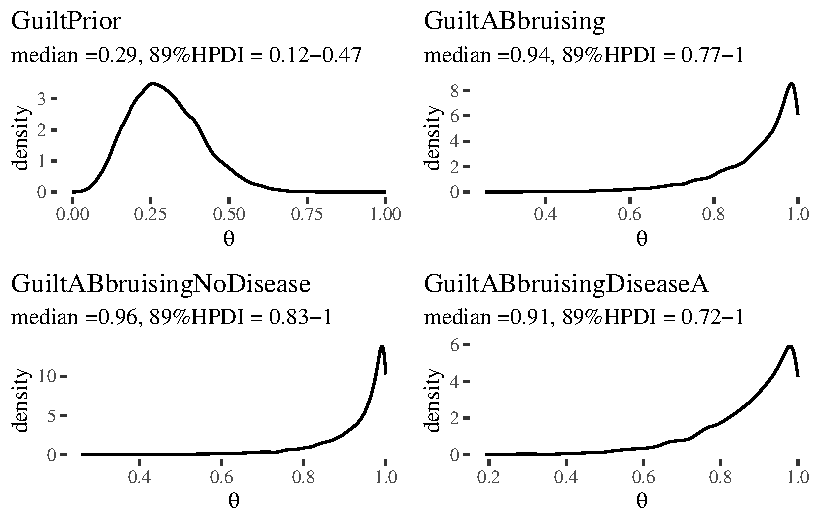
\includegraphics[width=0.9\textwidth,height=\textheight]{imp_philosophical_files/figure-pdf/fig-scwithhop2-1.pdf}

}

\caption{\label{fig-scwithhop2}Impact of incoming evidence in the Sally
Clark case.}

\end{figure}

One question that arises is how this approach relates to the standard
method of using likelihood ratios to report the value of the evidence.
On this approach, the conditional probabilities that are used in the
likelihood ratio calculations are estimated and come in a package with
an uncertainty about them. Accordingly, these uncertainties propagate:
to estimate the likelihood ratio while keeping track of the uncertainty
involved, we can sample probabilities from the selected distributions
appropriate for the conditional probabilities needed for the
calculations, then divide the corresponding samples, obtaining a sample
of likelihood ratios, thus approximating the density capturing the
recommended uncertainty about the likelihood ratio. Uncertainty about
likelihood ratio is just propagated uncertainty about the involved
conditional probabilities. For instance, we can use this tool to gauge
our uncertainty about the likelihood ratios corresponding to the signs
of bruising in son A and the presence of the symptoms of a potentially
lethal disease in son A (Figure~\ref{fig-sclrs}).

\begin{figure}[H]

{\centering 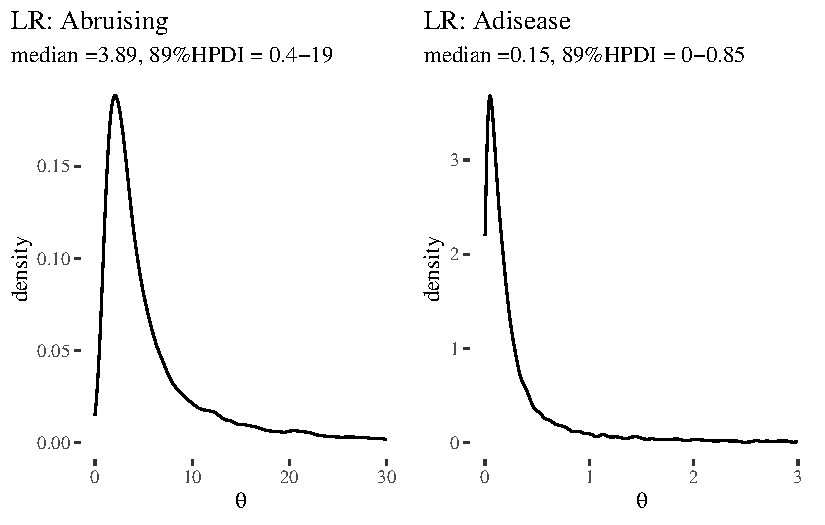
\includegraphics[width=0.9\textwidth,height=\textheight]{imp_philosophical_files/figure-pdf/fig-sclrs-1.pdf}

}

\caption{\label{fig-sclrs}Likelihood ratios forbruising and signs of
disease in child A in the Sally Clark case.}

\end{figure}

\hypertarget{conclusion}{%
\section{Conclusion}\label{conclusion}}

We have argued that higher-order probabilism outperforms both precise
and imprecise probabilism. It is able to model scenarios that the other
two cannot model, for example, the case of uneven bias. In addition,
higher-order probabilism does not fall prey to difficulties peculiar to
imprecise probabilism, such as belief inertia and the lack of proper
scoring rules. We have also identified a novel set of problems for
precise and imprecisse probabilism, mostly stemming from how to
evaluate, in the aggregate, multiple pieces of evidence. Here again,
higher-order probabilism fares better.

Some might dislike the idea of going higher-order for a numbere of
reasons, for exmaple, unnecessary complexity. This is a line taken by
Bradley, who refuses to go higher-order for the following reason:

\begin{quote}
Why is sets of probabilities the right level to stop the regress at? Why not sets of sets? Why not second-order probabilities? Why not single probability functions? This is something of a pragmatic choice. The further we allow this regress to continue, the harder it is to deal with these belief representing objects. So let's not go further than we need. 131-132\end{quote}

\noindent We have shown that given the difficulties of precise and
imprecise probabilism, we are not going further than we need in using
higher-order probabilities. The pragmatic concerns one might have are at
best unclear.

We should unnderscore that, mathematically, we do not propose anything
radically new. Concepts from the Bayesian toolkit that can model
higher-order uncertainty already exist. Our suggestion is that they have
been under-appreciated in formal epistemology and should be more widely
used. This is not to say that there is no need for any novel technical
work. For example, we still need a proper accuracy argument in defense
of higher-order probabilism. Will an agent who relies on higher-order
probabilities would accuracy-dominate one who relies on just first-order
probabilisties? We leave this as an open question. Another concern is
the lack of a clear semantics for higher-order probabilities. While a
more elaborate account is beyond the scope of this paper, the answer
should gesture at a modification of the framework of probabilistic
frames (Dorst, 2022b, 2022a). Start with a set of possible worlds \(W\).
Suppose you consider a class of probability distributions \(D\), a
finite list of atomic sentences \(q_1, \dots, q_2\) corresponding to
subsets of \(W\), and a selection of true probability hypotheses \(C\)
(think of the latter as omniscient distributions, \(C\subseteq D\), but
in principle this restriction can be dropped if need be). Each possible
world \(w\in W\) and a proposition \(p\subseteq W\) come with their true
probability distribution, \(C_{w,p}\in D\) corresponding to the true
probability of \(p\) in \(w\), and the distribution that the expert
assigns to \(p\) in \(w\), \(P_{w,p}\in D\). Then, various propositions
involving distributions can be seen as sets of possible worlds, for
instance, the proposition that the expert assigns \(d\) to \(p\) is the
set of worlds \(w\) such that
\(P_{w,p}=d\).\footnote{There is at least one important 
difference between this approach and that developed by Dorst. His framework is untyped, which allows for 
an enlightening discussion of the principle of reflection and alternatives to it. In this paper, we prefer 
to keep this complexity apart and use an explicitly typed set-up.}

\hypertarget{appendix-the-strict-propriety-of-i_kl}{%
\section*{\texorpdfstring{Appendix: the strict propriety of
\(I_{kl}\)}{Appendix: the strict propriety of I\_\{kl\}}}\label{appendix-the-strict-propriety-of-i_kl}}
\addcontentsline{toc}{section}{Appendix: the strict propriety of
\(I_{kl}\)}

The fact that \(I_{KL}\) is strictly proper as applied to second-order
probabilities is not very surprising. However, in the existing
literature, the proof is not usually explicitly given, and some of the
pieces are not present in philosophical literature. So we tried to
include the whole chain of thought, warning that some of these results
are already known and all we did was making the proofs more presentable,
and pointing out new elements in the reasoning. Let us start with a
definition of concavity.

\begin{definition}[concavity]

A function $f$ is convex over an interval $(a,b)$ just in case for all  $x_1, x_2\in (a,b)$ and 
$0 \leq \lambda \leq 1$ we have:
\begin{align*}
f(\lambda x_1 + (1-\lambda)x_2) \leq \lambda f(x_1) + (1-\lambda)f(x_2)
\end{align*}

\noindent A function $f$  is concave just in case:
\begin{align*}
f(\lambda x_1 + (1-\lambda)x_2) \geq \lambda f(x_1) + (1-\lambda)f(x_2)
\end{align*}
\noindent A function $f$  is strictly concave just in case the equality holds only if either $\lambda = 0$ or $\lambda = 1$.
\end{definition}

For us it is important that if a function is twice differentiable on an
interval, then it is (strictly) concave just in case its second
derivative is non-positive (negative). In particular, as
\((\log_2(x))'' = -\frac{1}{x^2 ln(2)}\), \(\log_2\) is strictly concave
over its
domain.\footnote{I line with the rest of the paper, we'll work with $\log$ base 2. We could equally well use any other basis.}
\todo{NL: Why ''?}

\begin{lemma}[Jensen's inequality]
If $f$ is concave, and $g$ is any function of a random variable, $\mathbb{E}(f(g(x))) \leq f(\mathbb{E}(g(x)))$. If $f$ is 
strictly concave, the equality holds only if $g(x) = \mathbb{E} g(x)$, that is, if $g(x)$ is constant everywhere.
\end{lemma}

\begin{proof}
For the base case consider a two-point mass probability function. Then,
\begin{align*}
p_1f(g(x_1))+ p_2f(g(x_2)) &\leq f(p_1g(x_1) + p_2g(x_2))
\end{align*}
\noindent follows directly from the definition of concativity, if we take $\lambda = p_1$, $(1-\lambda)=p_2$,
 and substitute $g(x_1)$ and $g(x+2)$ for $x_1$ and $x_2$.



Now, suppose that  $ p_1f(g(x_1))+ p_2f(g(x_2)) = f(p_1g(x_1) + p_2g(x_2))$ and that   $f$ is strictly concave.
 That means either $(p_1 = 1\wedge p_2 = 0)$, or $(p_1 = 0 \wedge p_2 =1)$. Then either $x$ always takes
  value $x_1$, in the former case, or always takes value $x_2$, in the latter
   case. $\mathbb{E} g (x) =  p_1 g(x_1) + p_2 g(x_2)$, which equals  $g(x_1)$ in the former case and $g(x_2)$ in the latter.


Now suppose Jensen's inequality and the consequence of strict contativity holds for $k-1$ mass points. 
Write $p_i' = \frac{p_i}{1-p_k}$ for $i = 1, 2, \dots, k-1$. We now reason:
\begin{align*}
\sum_{i=1}^k p_i f(g(x_i)) & =
 p_kf(g(x_k)) + (1-p_k)\sum_{i =1}^{k-1}p_i'f(g(x_i)) &\\
 & \leq p_k f(g(x_k)) + (1-p_k)f\left( \sum_{i = 1}^{k=i}p_i' g(x_i) \right) & \mbox{\footnotesize by 
 the induction hypothesis}\\ &\leq f\left( p_k(g(x_k)) + (1-p_k)\sum_{i = 1}^{k-1} p_i' g(x_i)\right) & 
 \mbox{\footnotesize by the base case} \\
 & = f \left( \sum_{i}^k p_i g(x_i)\right)
 \end{align*}

Notice also that at the induction hypothesis application stage we know that the equality holds only if 
$p_k =1 \vee p+k = 0$. In the former case $g(x)$ always takes value $x_k = \mathbb{E} g(x)$. In the latter case,
 $p_k$ can be safely ignored and $\sum_{i=1}^{k}p_ig(x_i) = \sum_{i=1}^{k-1}p'g(x_i)$ and by the induction 
 hypothesis we already know that $\mathbb{E} g(x) = g(x)$.


\end{proof}

In particular, the claim holds if we take \(g(x)\) to be
\(\frac{q(x)}{p(x)}\) (were both \(p\) and \(q\) are probability mass
functions), and \(f\) to be \(\log_2\). Then, given that \(A\) is the
support set of \(p\), we have: \begin{align*}
\sum_{x\in A}p(x) \log_2 \frac{q(x)}{p(x)} & \leq \log_2 \sum_{x\in A}p(x)\frac{q(x)}{p(x)}
\end{align*}

\noindent Moreover, the equality holds only if \(\frac{q(x)}{p(x)}\) is
constant, that is, only if \(p\) and \(q\) are the same pmfs. Let's use
this in the proof of the following lemma.

\begin{lemma}[Information inequality] For two probability mass functions $p, q$, $\dkl(p,q)\geq 0$ with 
equality iff $p=q$.
\end{lemma}

\begin{proof}
Let $A$ be the support set of $p$, and let $q$ be a probability mass function whose support is $B$.
\begin{align*}
- \dkl(p,q) & = - \sum_{x\in A}p(x) \log_2 \frac{p(x)}{q(x)}& \mbox{\footnotesize (by definition)} \\
&  =  \sum_{x\in A}p(x)  - \left(\log_2 p(x) - \log_2 q(x)\right)& \\
&  =  \sum_{x\in A}p(x)   \left(\log_2 q(x) - \log_2 p(x)\right)& \\
& =  \sum_{x\in A} p(x) \log_2 \frac{q(x)}{p(x)}& \\
& \leq \log_2 \sum_{x\in A} p(x)\frac{q(x)}{p(x)} & \mbox{\footnotesize by Jensen's inequality}\\
& \mbox{(and the equality holds only if $p = q$)}\\
& = \log_2 \sum_{x\in A} q(x)  & \\
& \leq \log_2 \sum_{x\in B} q(x) & \\
& = log (1)  = 0 &\\
\end{align*}
\end{proof}

Observe now that \(\dkl\) can be decomposed in terms of cross-entropy
and entropy.

\begin{lemma}[decomposition] $\dkl = H(p,q) - H(p)$. \end{lemma}

\begin{proof}
\begin{align*}
\dkl (p, q) & = \sum_{p_{i}} \left( \log_2 p_i - \log_2 q_i \right) \\
& =   - \sum_{p_{i}}\left( \log_2 q_{i} - \log_2 p_{i} \right) \\
& = - \sum_{p_{i}} \log_{2} q_{i} - \sum_{p_{i}} - \log_{2} p_{i}   \\
& -  \underbrace{- \sum_{p_{i}} \log_2 q_{i}}_{H(p,q)}    - \underbrace{- \sum_{p_i}  \log_2 p_{i}}_{H(p)}
\end{align*}
\end{proof}

With information inequality this easily entails Gibbs' inequality:

\begin{lemma}[Gibbs' inequality] $H(p,q) \geq H(p)$ with identity only if $p = q$.
\end{lemma}

We are done with our theoretical set-up, which is already common
knowledge, except presented in an orderly manner in one place. Now we
present our argument for the cliam that the above entails the propriety
of \(I_{KL}\). First, let's systematize the notation. Consider a
discretization of the parameter space \([0,1]\) into \(n\) equally
spaced values \(\theta_1, \dots, \theta_n\). For each \(i\) the
``true'\,' second-order distribution if the true parameter indeed is
\(\theta_i\)---we'll call it the indicator of \(\theta_i\)--- which is
defined by \begin{align*}
Ind^k(\theta_i) & = \begin{cases} 1 & \mbox{if } \theta_i = \theta_k\\
                        0 & \mbox{otherwise}  \end{cases}
\end{align*} \noindent We will write \(Ind^k_i\) instead of
\(Ind^k(\theta_i)\).

Now consider a probability distribution \(p\) over this parameter space,
assigning probabilities \(p_1, \dots, p_n\) to
\(\theta_1, \dots, \theta_n\) respectively. It is to be evaluated in
terms of inaccuracy from the perspective of a given `true' value
\(\theta_k\). The inaccuracy of \(p\) if \(\theta_k\) is the `true'
value, is the divergence between \(Ind^k\) and \(p\).

\begin{align*}
I_{KL}(p, \theta_k) & = D_\text{KL}(Ind^k||p) \\
& = \sum_{i=1}^n Ind^k_i \left( \log_2 Ind^k_i - \log_2 p_i \right)
\end{align*} Note now that for \(j \neq k\) we have \(Ind^k_j = 0\) and
so \(Ind^k_j \left( \log_2 Ind^k_j - \log_2 p_j \right)=0\). Therefore
we continue: \begin{align*}
& = Ind^k_k \left( \log_2 Ind^k_k - \log_2 p_k \right)
\end{align*} Further, \(Ind^k_k= 1\) and therefore
\(\log_2 Ind^k_k =0\), so we simplify: \begin{align*}
& =  - \log_2 p_k
\end{align*}

\noindent Now, let's think about expected values. First, what is the
inaccuracy of \(p\) as expected by \(p\),
\(\mathbb{E}I_{\text{DK}}(p,p)\)?

\begin{align*}
\mathbb{E}I_{\text{DK}}(p,p) & = \sum_{i =1}^n p_i I_{\text{DK}}(p, \theta_k) \\
& = \sum_{i =1}^n  p_i - \log_2 p_k \\
& = - \sum_{i =1}^n  p_i  \log_2 p_k = H(p)
\end{align*}

\noindent Analogously, the inaccuracy of \(q\) as expected from the
perspective of \(p\) is:

\begin{align*}
\mathbb{E}I_{\text{DK}}(p, q) & =   \sum_{i =1}^n p_i \left( - \log_2 q_i\right)\\
& = -  \sum_{i =1}^n p_i  \log_2 q_i = H(p,q)
\end{align*}

But that means, by Gibbs' inequality, that
\(\mathbb{E}I_{\text{DK}}(p,q) \geq \mathbb{E}I_{\text{DK}}(p,p)\)
unless \(p=q\), which completes the proof.

\hypertarget{references}{%
\section*{References}\label{references}}
\addcontentsline{toc}{section}{References}

\hypertarget{refs}{}
\begin{CSLReferences}{1}{0}
\leavevmode\vadjust pre{\hypertarget{ref-Bingham2021PPwithoutTears}{}}%
Bingham, E., Koppel, J., Lew, A., Ness, R., Tavares, Z., Witty, S., \&
Zucker, J. (2021). Causal probabilistic programming without tears.
\emph{Proceedings of the Third Conference on Probabilistic Programming}.

\leavevmode\vadjust pre{\hypertarget{ref-bradley2012scientific}{}}%
Bradley, S. (2012). \emph{Scientific uncertainty and decision making}
(PhD thesis). London School of Economics; Political Science (University
of London).

\leavevmode\vadjust pre{\hypertarget{ref-bradley2019imprecise}{}}%
Bradley, S. (2019). {Imprecise Probabilities}. In E. N. Zalta (Ed.),
\emph{The {Stanford} encyclopedia of philosophy} ({S}pring 2019).
\url{https://plato.stanford.edu/archives/spr2019/entries/imprecise-probabilities/};
Metaphysics Research Lab, Stanford University.

\leavevmode\vadjust pre{\hypertarget{ref-CampbellMoore2020accuracy}{}}%
Campbell-Moore, C. (2020). \emph{Accuracy and imprecise probabilities}.

\leavevmode\vadjust pre{\hypertarget{ref-Carr2020impreciseEvidence}{}}%
Carr, J. R. (2020). Imprecise evidence without imprecise credences.
\emph{Philosophical Studies}, \emph{177}(9), 2735--2758.
\url{https://doi.org/10.1007/s11098-019-01336-7}

\leavevmode\vadjust pre{\hypertarget{ref-deadman1984fiber2}{}}%
Deadman, H. A. (1984a). Fiber evidence and the wayne williams trial
(conclusion). \emph{FBI L. Enforcement Bull.}, \emph{53}, 10--19.

\leavevmode\vadjust pre{\hypertarget{ref-deadman1984fiber1}{}}%
Deadman, H. A. (1984b). Fiber evidence and the wayne williams trial
(part i). \emph{FBI L. Enforcement Bull.}, \emph{53}, 12--20.

\leavevmode\vadjust pre{\hypertarget{ref-Dorst2022evidence}{}}%
Dorst, K. (2022a). Higher-order evidence. In M. Lasonen-Aarnio \& C.
Littlejohn (Eds.), \emph{The routledge handbook for the philosophy of
evidence}. Routledge.

\leavevmode\vadjust pre{\hypertarget{ref-Dorst2022higher-order}{}}%
Dorst, K. (2022b). Higher-order uncertainty. In M. Skipper \& A. S.
Petersen (Eds.), \emph{Higher-order evidence: New essays}.

\leavevmode\vadjust pre{\hypertarget{ref-Lee2017impreciseEpistemology}{}}%
Elkin, L. (2017). \emph{Imprecise probability in epistemology} (PhD
thesis). Ludwig-Maximilians-Universit{ä}t;
Ludwig-Maximilians-Universität München.

\leavevmode\vadjust pre{\hypertarget{ref-Fenton2018Risk}{}}%
Fenton, N., \& Neil, M. (2018). \emph{Risk assessment and decision
analysis with bayesian networks}. Chapman; Hall.

\leavevmode\vadjust pre{\hypertarget{ref-VanFraassen2006vague}{}}%
Fraassen, B. C. V. (2006). Vague expectation value loss.
\emph{Philosophical Studies}, \emph{127}(3), 483--491.
\url{https://doi.org/10.1007/s11098-004-7821-2}

\leavevmode\vadjust pre{\hypertarget{ref-Gardenfors1982unreliable}{}}%
Gärdenfors, P., \& Sahlin, N.-E. (1982). Unreliable probabilities, risk
taking, and decision making. \emph{Synthese}, \emph{53}(3), 361--386.
\url{https://doi.org/10.1007/bf00486156}

\leavevmode\vadjust pre{\hypertarget{ref-GneitRafter2007}{}}%
Gneiting, T., \& Raftery, A. E. (2007). Strictly proper scoring rules,
prediction, and estimation. \emph{Journal of the American Statistical
Association}, \emph{102}(477), 359--378.
\url{https://doi.org/10.1198/016214506000001437}

\leavevmode\vadjust pre{\hypertarget{ref-HersbachDecomp2000}{}}%
Hersbach, H. (2000). Decomposition of the continuous ranked probability
score for ensemble prediction systems. \emph{Weather and Forecasting},
\emph{15}(5), 559--570.
https://doi.org/\url{https://doi.org/10.1175/1520-0434(2000)015\%3C0559:DOTCRP\%3E2.0.CO;2}

\leavevmode\vadjust pre{\hypertarget{ref-joyce2005probabilities}{}}%
Joyce, J. M. (2005). How probabilities reflect evidence.
\emph{Philosophical Perspectives}, \emph{19}(1), 153--178.

\leavevmode\vadjust pre{\hypertarget{ref-Kaplan1968decision}{}}%
Kaplan, J. (1968). Decision theory and the fact-finding process.
\emph{Stanford Law Review}, \emph{20}(6), 1065--1092.

\leavevmode\vadjust pre{\hypertarget{ref-keynes1921treatise}{}}%
Keynes, J. M. (1921). \emph{A treatise on probability, 1921}. London:
Macmillan.

\leavevmode\vadjust pre{\hypertarget{ref-kruschke2015doing}{}}%
Kruschke, J. (2015). \emph{Doing bayesian data analysis (second
edition)}. Boston: Academic Press.

\leavevmode\vadjust pre{\hypertarget{ref-Kyburg1961}{}}%
Kyburg, H. E. (1961). \emph{Probability and the logic of rational
belief}. Wesleyan University Press.

\leavevmode\vadjust pre{\hypertarget{ref-kyburg2001uncertain}{}}%
Kyburg Jr, H. E., \& Teng, C. M. (2001). \emph{Uncertain inference}.
Cambridge University Press.

\leavevmode\vadjust pre{\hypertarget{ref-Levi1974ideterminate}{}}%
Levi, I. (1974). On indeterminate probabilities. \emph{The Journal of
Philosophy}, \emph{71}(13), 391. \url{https://doi.org/10.2307/2025161}

\leavevmode\vadjust pre{\hypertarget{ref-Levi1980enterprise}{}}%
Levi, I. (1980). \emph{The enterprise of knowledge: An essay on
knowledge, credal probability, and chance}. MIT Press.

\leavevmode\vadjust pre{\hypertarget{ref-Mayo-Wilson2016scoring}{}}%
Mayo-Wilson, C., \& Wheeler, G. (2016). Scoring imprecise credences: A
mildly immodest proposal. \emph{Philosophy and Phenomenological
Research}, \emph{92}(1), 55--78.
\url{https://doi.org/10.1111/phpr.12256}

\leavevmode\vadjust pre{\hypertarget{ref-Pettigrew2012Epistemic-Utili}{}}%
Pettigrew, R. (2012). \emph{Epistemic utility and norms for credences}.

\leavevmode\vadjust pre{\hypertarget{ref-Rinard2013against}{}}%
Rinard, S. (2013). Against radical credal imprecision. \emph{Thought: A
Journal of Philosophy}, \emph{2}(1), 157--165.
\url{https://doi.org/10.1002/tht3.84}

\leavevmode\vadjust pre{\hypertarget{ref-Schoenfield2017accuracy}{}}%
Schoenfield, M. (2017). The accuracy and rationality of imprecise
credences. \emph{Noûs}, \emph{51}(4), 667--685.
\url{https://doi.org/10.1111/nous.12105}

\leavevmode\vadjust pre{\hypertarget{ref-seidenfeld2012forecasting}{}}%
Seidenfeld, T., Schervish, M., \& Kadane, J. (2012). Forecasting with
imprecise probabilities. \emph{International Journal of Approximate
Reasoning}, \emph{53}, 1248--1261.
\url{https://doi.org/10.1016/j.ijar.2012.06.018}

\leavevmode\vadjust pre{\hypertarget{ref-Sturgeon2008grain}{}}%
Sturgeon, S. (2008). Reason and the grain of belief. \emph{No{û}s},
\emph{42}(1), 139--165. Retrieved from
\url{http://www.jstor.org/stable/25177157}

\leavevmode\vadjust pre{\hypertarget{ref-walley1991statistical}{}}%
Walley, P. (1991). \emph{Statistical reasoning with imprecise
probabilities}. Chapman; Hall London.

\end{CSLReferences}



\end{document}
